\documentclass[
fontsize=10pt, % Font size
pagesize, % Write page size to dvi or pdf
parskip=half-, % Paragraphs separated by half a line
]{article} % KOMA script (article)

\linespread{1.12} % Increase line spacing for readability

% ----------------------------------------------------------------------
% Colors
\usepackage{xcolor}	 % Required for custom colors
% Define a few colors for making text stand out within the presentation
\definecolor{colorbg}{RGB}{60,60,100}
\definecolor{myblue}{RGB}{34,31,217}
\definecolor{mybrown}{RGB}{139,69,19}
\definecolor{myyellow}{RGB}{236,171,21}
\definecolor{mygreen}{RGB}{5,102,8}
\definecolor{myred}{RGB}{255,66,56}
\definecolor{mygray}{RGB}{160,160,160}
\definecolor{mypurple}{RGB}{186,85,211}

\newcommand \temp {\color{red}[[TEMP]]}
\newcommand \finTemp {\color{black}[[ENDTEMP]]}
% Use these colors within the presentation by enclosing text in the commands below
\newcommand*{\colorbg}[1]{\textcolor{colorbg}{#1}}
\newcommand*{\myblue}[1]{\textcolor{myblue}{#1}}
\newcommand*{\mybrown}[1]{\textcolor{mybrown}{#1}}
\newcommand*{\myred}[1]{\textcolor{myred}{#1}}
\newcommand*{\myyellow}[1]{\textcolor{myyellow}{#1}}
\newcommand*{\mygray}[1]{\textcolor{mygray}{#1}}
\newcommand*{\mypurple}[1]{\textcolor{mypurple}{#1}}
\newcommand*{\mygreen}[1]{\textcolor{mygreen}{#1}}
\newcommand   \Esp    {\mathbb{E}}
\newcommand \SnMC     {\hat{S}_{n}^{\rm MC}}
\newcommand \SnCV     {\hat{S}_{n}^{\rm cv}}
\newcommand \SnSt     {\hat{S}_{n}^{\rm str}}
\newcommand \DDelta   {\bm{\Delta}}
\newcommand \uDelta   {\underline{\Delta}}
\newcommand \FD       {F_{\uDelta}}
\usepackage{mathtools}
\DeclarePairedDelimiter{\ceil}{\lceil}{\rceil}
% ----------------------------------------------------------------------
% Margins
\usepackage[ % Page margins settings
paperwidth=128mm,
paperheight=96mm,
includeheadfoot,
top=3.5mm,
bottom=1mm,
left=5.5mm,
right=5.5mm,
headsep=5.5mm,
headheight=8mm,
footskip=7mm
]{geometry}
% ----------------------------------------------------------------------

% Fonts
\usepackage[T1]{fontenc}	 % For correct hyphenation and T1 encoding
\usepackage{lmodern} % Default font: latin modern font
%\usepackage{fourier} % Alternative font: utopia
%\usepackage{charter} % Alternative font: low-resolution roman font
\renewcommand{\familydefault}{\sfdefault} % Sans serif - this may need to be commented to see the alternative fonts

\usepackage{fancyhdr}
\usepackage{amssymb,amsfonts,amsthm,amsmath} % Required for theorem environments
\usepackage[mathscr]{euscript}

\usepackage{bm, bbm, dsfont} % Required for bold math symbols (used in the footer of the slides)
\usepackage{enumerate}
\usepackage{graphicx,psfrag}
\graphicspath{{./figs/}}
\usepackage{tikz} % Required for colored boxes
\usetikzlibrary{positioning,calc}
\usepackage{booktabs} % Required for horizontal rules in tables
\usepackage{multicol} % Required for creating multiple columns in slides
\usepackage{enumitem}
\usepackage{lastpage} % For printing the total number of pages at the bottom of each slide
\usepackage[english]{babel} % Document language - required for customizing section titles
\usepackage{microtype} % Better typography
\usepackage{tocstyle} % Required for customizing the table of contents
\usepackage{ulem}
\usepackage{siunitx}
\usepackage{booktabs}
%\usepackage{chapterbib}
\usepackage[sort,comma,authoryear,round]{natbib}
\usepackage{caption}
\usepackage{subcaption}
\captionsetup[table]{labelformat=empty}
\usepackage{ccicons}
\usepackage{algorithm}
\usepackage{algpseudocode}
\usepackage{multicol}
\usepackage{siunitx}
\usepackage{arydshln}
\DeclareMathOperator{\Var}{Var}
\DeclareMathOperator{\lognormal}{Lognormal}
\DeclareMathOperator{\weibull}{Weibull}
\DeclareMathOperator{\poisson}{Poisson}
% ----------------------------------------------------------------------
\usepackage{notations}
\usepackage{adjustbox}
\usetikzlibrary{arrows.meta}
\usepackage{titlesec}
\setcounter{secnumdepth}{4}

\titleformat{\paragraph}
{\normalfont\normalsize\bfseries}{\theparagraph}{1em}{}
\titlespacing*{\paragraph}
{0pt}{3.25ex plus 1ex minus .2ex}{1.5ex plus .2ex}
% ----------------------------------------------------------------------

% Sets vertical centering of slide contents with increased space between paragraphs/lists
\makeatletter
\renewcommand*{\@textbottom}{\vskip \z@ \@plus 1fil}
\newcommand*{\@texttop}{\vskip \z@ \@plus .5fil}
\addtolength{\parskip}{\z@\@plus .04fil}
\makeatother
\setlength{\parindent}{0pt}
% Remove page numbers and the dots leading to them from the outline slide
\makeatletter
\newtocstyle[noonewithdot]{nodotnopagenumber}{\settocfeature{pagenumberbox}{\@gobble}}
\makeatother
\usetocstyle{nodotnopagenumber}
\setcounter{tocdepth}{1}
%\AtBeginDocument{\renewcaptionname{english}{\contentsname}{\Large
%Outline}} % Change the name of the table 

% ----------------------------------------------------------------------

\pagestyle{fancy} \fancyhf{} \renewcommand{\headrulewidth}{0.5pt}
\renewcommand{\footrulewidth}{0.0pt}
\rhead{\scriptsize\thepage/\pageref{LastPage}}
\lfoot{
\begin{tikzpicture}
%    \draw [color=mygray] (0,0) -- (0.9\paperwidth,0);
    \node [anchor=north west, inner sep=0pt] at (0,-2mm)
    {\scriptsize\mygray{\hspace{0.1cm}\myauthor~\raisebox{0.2mm}{$\bm{\vert}$}~\runninghead~\raisebox{0.2mm}{$\bm{\vert}$}~ArtiSaneFood~\raisebox{0.2mm}{$\bm{\vert}$}~\myuni~\raisebox{0.2mm}{$\bm{\vert}$}~\mydate}};
  \end{tikzpicture}}

\def\headerbar{\vbox{%

\begin{tikzpicture}
  \node at (0, 0)
  [anchor=north west, rectangle, fill, inner
  sep=0pt, minimum width=0.93\paperwidth, minimum
  height=1.5pt, top color=colorbg, bottom
  color=colorbg]{};
\end{tikzpicture}}}
 
\def\footbar{
\begin{tikzpicture}
  \node at (-3.7cm, 0)[anchor=north west, rectangle,fill,inner sep=0pt,minimum
  width=0.93\paperwidth,minimum height=1pt,top color=colorbg,bottom
  color=colorbg]{}; % Green bar
  \node at (-3.7cm,-1.5mm)[anchor=north west, inner sep=0pt] {\scriptsize \myauthor\ \raisebox{0.2mm}{$\bm{\vert}$}\ \myuni}; % Left side text}
%  \draw (0,0) -- (1,0);
\end{tikzpicture}}
%\ifoot{\footbar}


%------------------------------------------------
% Section spacing - deeper section titles are given less space due to lesser importance
\usepackage{titlesec} % Required for customizing section spacing
\titlespacing{\section}{0mm}{0mm}{6mm} % Lengths are: left, before, after
\titlespacing{\subsection}{0mm}{0mm}{5mm} % Lengths are: left, before, after
\titlespacing{\subsubsection}{0mm}{0mm}{0mm} % Lengths are: left, before, after
\setcounter{secnumdepth}{2} % How deep sections are numbered, set to no
                            % numbering by default - change to 1 for
                            % numbering sections, 2 for numbering
                            % sections and subsections, etc
\titleformat{\subsection}{\normalfont\large\bfseries}{}{0pt}{}
%------------------------------------------------

%------------------------------------------------
% Theorem style
\newtheoremstyle{mythmstyle} % Defines a new theorem style used in this template
{0.5em} % Space above
{0.5em} % Space below
{} % Body font
{} % Indent amount
{\sffamily\bfseries} % Head font
{} % Punctuation after head
{\newline} % Space after head
{\thmname{#1}\ \thmnote{(#3)}} % Head spec
	
\theoremstyle{mythmstyle} % Change the default style of the theorem to the one defined above
\newtheorem{theorem}{Theorem}[section] % Label for theorems
\newtheorem{remark}[theorem]{Remark} % Label for remarks
%\newtheorem{algorithm}[theorem]{Algorithm} % Label for algorithms
\makeatletter % Correct qed adjustment
%------------------------------------------------

%------------------------------------------------
% The code for the box which can be used to highlight an element of a slide (such as a theorem)
\newcommand*{\mybox}[2]{ % The box takes two arguments: width and content
\par\noindent
\begin{tikzpicture}[mynodestyle/.style={rectangle,draw=colorbg,thick,inner sep=2mm,text justified,top color=white,bottom color=white,above}]\node[mynodestyle,at={(0.5*#1+2mm+0.4pt,0)}]{ % Box formatting
\begin{minipage}[t]{#1}
#2
\end{minipage}
};
\end{tikzpicture}
\par\vspace{-1.3em}}

\newcommand{\ngr}{\newpage\addtocounter{page}{-1}}
\DeclareMathOperator{\score}{score}
\usepackage[most]{tcolorbox}
\colorlet{LightLavender}{blue!25}
\tcbset{on line, 
        boxsep=4pt, left=0pt,right=0pt,top=0pt,bottom=0pt,
        colframe=white,colback=LightLavender,  
        highlight math style={enhanced}
        }
		
%-----------------------------------------------------------------------
%	PRESENTATION INFORMATION
%-----------------------------------------------------------------------

\newcommand*{\mytitle}{PhD defence} % Title
\newcommand*{\runninghead}{PhD defense} % Running head displayed on almost all slides
\newcommand*{\myauthor}{Subhasish Basak} % Presenters name(s)
\newcommand*{\mydate}{March 20, 2024} % Presentation date
\newcommand*{\myuni}{ANSES - L2S - Université Paris Saclay} % University or department

\usepackage[hidelinks]{hyperref} 
\hypersetup{%
  bookmarksnumbered, %
  bookmarksdepth=2, %
  colorlinks=false, %
  breaklinks, %
  pdfborder=0 0 0, %
  pdftitle={\mytitle}, %
  pdfauthor={Subhasish Basak}, %
  pdfkeywords={}%
}

%-----------------------------------------------------------------------
\begin{document}
\thispagestyle{empty} % No slide header and footer
% Define box and box title style

\tikzstyle{titlebox} = [fill=colorbg, rectangle, inner sep=10pt, inner ysep=16pt]
\tikzstyle{fancytitle} =[fill=red, text=white]
\hspace{-8mm}%
\begin{tikzpicture}
\node [titlebox] (box){%
    \begin{minipage}{\paperwidth}
      \begin{center}
        \color{white}\sffamily 

        {\large Multipathogen quantitative risk assessment in raw milk soft cheese,
		monotone integration and Bayesian optimization} 
	      \vskip 0.5cm 
	      \small
		  Subhasish Basak$^{1, 2}$
	      \vskip 0.45cm
		  PhD defense
	      \vskip 0.0cm
	      March 20, 2024 - Paris-Saclay, France
		  \vskip 0.45cm
		  Supervised by \\
	      Julien Bect$^2$, Laurent Guillier$^1$, Fanny Tenenhaus-Aziza$^3$ \& Emmanuel Vazquez$^2$ 
	 \vskip 0.3cm
	 {\fontsize{6.5}{6.5}\selectfont 1. Agence Nationale de Sécurité Sanitaire (ANSES), Maison-Alfort, France}
	 \vskip -0.15cm
	 {\fontsize{6.5}{6.5}\selectfont 2. Université Paris-Saclay, CNRS, CentraleSupeléc, L2S, Gif-sur-yvette, France}
	 \vskip -0.15cm
	 {\fontsize{6.5}{6.5}\selectfont 3. Centre national interprofessionnel de l'économie laitière (CNIEL), Paris, France}
	 \vspace{-0.6cm}
      \end{center}
    \end{minipage}
};
%\node[fancytitle, right=10pt] at (box.north west) {A fancy title};
%\node[fancytitle, rounded corners] at (box.east) {$\clubsuit$};
\end{tikzpicture}
\clearpage
% ----------------------------------------------------------------------
%\thispagestyle{empty}
\vskip-2cm
\begin{center}
	\vskip-5cm
	\begin{minipage}[c]{\linewidth}
    \centering
	\includegraphics[scale=0.11]{images/logos/prima.png}
	\hspace{9mm}%
	\includegraphics[scale=0.095]{images/logos/artisane.png}
        \hspace{8mm}%
	\includegraphics[scale=0.3]{images/logos/anr.png}
	\hspace{9mm}%
	\vskip 2cm
	\end{minipage}
	\par
\end{center}
\vspace{0.05cm}
%\small
\begin{center}
	%This work is part of the \myblue{ArtiSaneFood} project (grant : 
	%ANR-18-PRIM-0015), supported by the \myblue{PRIMA} 
	%program of the \myblue{European Union}.
	%\textbf{European project ArtiSaneFood}
	%\par
	Innovative Bio-interventions and Risk Modelling Approaches for 
	Ensuring Microbial Safety and Quality of Mediterranean Artisanal 
	Fermented Foods
\end{center}
\vspace{0.02cm}
\begin{center}
	\begin{minipage}[c]{\linewidth}
    \centering
	\includegraphics[scale=0.25]{images/logos/ipb.png}
	\hspace{3mm}%
	\includegraphics[scale=0.18]{images/logos/anses.png}
	\hspace{5mm}%
	\includegraphics[scale=0.17]{images/logos/cniel.jpg}
        \hspace{5mm}%
	\includegraphics[scale=0.24]{images/logos/uco.png}
        \hspace{2mm}%
	\includegraphics[scale=0.17]{images/logos/ub.png}	
        \hspace{4mm}%
	\end{minipage}
	\par
\end{center}
\begin{center}
	\begin{minipage}[c]{\linewidth}
    \centering
	\includegraphics[scale=0.33]{images/logos/zohr.png}
	\hspace{7mm}%
	\includegraphics[scale=0.35]{images/logos/aua.png}
        \hspace{2mm}%
	\includegraphics[scale=0.35]{images/logos/manouba1.png}
	\hspace{2mm}%
	\end{minipage}
	\par
\end{center}
\newpage
% ----------------------------------------------------------------------
%\thispagestyle{empty}
\vspace{-8mm}
\Large 
\textbf{ArtiSaneFood France}
\normalsize
\begin{itemize}
	\item \myblue{Potential pathogen contamination} - 
		\myred{Raw milk soft cheese} 
		\par 
		``fromages au lait cru'' - milk heated $< 40$°C
	\begin{itemize}
		\item[]1. Shiga toxin-producing \textit{Escherichia coli} 
			(STEC)
			%$\rightarrow$ Haemolytic Uremic 
			%Syndrome
		\item[]2. \textit{Salmonella} %$\rightarrow$ 
			%Salmonellosis
		\item[]3. \textit{Listeria monocytogenes}
			%$\rightarrow$ Listeriosis
	\end{itemize}
\end{itemize}
%\vspace{0.02cm}
\begin{center}
	\begin{minipage}[c]{\linewidth}
    \centering
	\includegraphics[scale=0.18]{images/logos/anses.png}
	\hspace{5mm}%
	\includegraphics[scale=0.17]{images/logos/cniel.jpg}
        \hspace{5mm}%
	\includegraphics[scale=0.18]{images/logos/actalia.jpg}
        \hspace{5mm}%
	\includegraphics[scale=0.25]{images/logos/aop.jpg}
        \hspace{1mm}%
	\includegraphics[scale=0.25]{images/logos/cnaol.jpg}
        \hspace{5mm}%
	\end{minipage}
	\par
\end{center}
\begin{center}
	\begin{minipage}[c]{\linewidth}
    \centering
	\includegraphics[scale=0.2]{images/logos/laitcru.png}
	\hspace{2mm}%
	\includegraphics[scale=0.05]{images/logos/cs.jpg}
	\hspace{2mm}%
	\includegraphics[scale=0.03]{images/logos/cnrs.png}
        \hspace{2mm}%
	\includegraphics[scale=0.2]{images/logos/l2s.png}
	\hspace{2mm}%
	\end{minipage}
	\par
\end{center}
\newpage
%-----------------------------------------------------------------------
%\Large{\textbf{Context}}
%\normalsize
\begin{figure}[H]
  	\centering
		\includegraphics[width=0.8\textwidth]{images/conso/pic.png}
\end{figure}
\begin{itemize}
	\item \myblue{Intervention practices} - \myred{Food safety 
		regulations}
		\vspace{-1.7mm}
	\begin{multicols}{2}
	            \item[] \tcbox{Test farm milk}
		    \item[] $\rightarrow$ everyday ? every $10$ days ? 
		    \item[] $\rightarrow$ \textit{E. coli} contamination 
			    level ? 
		    \item[] \tcbox{Test cheese batches}
		    \item[] $\rightarrow$ Test every batch ? (expensive!)
		    \item[] $\rightarrow$ How many samples to test ? 
        \end{multicols}
\end{itemize}
\newpage 
%-----------------------------------------------------------------------
\Large{\textbf{Context}}
\normalsize
\begin{itemize}
	\item \myblue{Goal}: \myred{Ensure the safety of raw milk soft 
		cheese!} 
		\begin{itemize}
			%\item[]$\rightarrow$ Improve
			%	intervention strategies 
			%\item[]$\rightarrow$ Reduce \myred{risk} of 
			%	illnesses and \myred{cost} of 
			%	interventions
			\item Optimize the interventions for 3 pathogens 
				simultaneously	
		\end{itemize}
	\item \myblue{Quantities to $\searrow$ minimize}
	\vspace{-0.4cm}
		\begin{center}
			\tcbox{Risk for consumer} 
			\par
			trade $\uparrow$ $\downarrow$ off
			\par
			\tcbox{Cost for producer}
		\end{center}
	\vspace{-0.2cm}
	\item \myblue{Multiobjective optimization} - \myred{optimal 
		intervention parameters}
	\begin{itemize}
		\item[] \myblue{$p_{\rm milk}$}, \myblue{$p_{\rm cheese}$}: 
			proportion of farm milk/cheese batches tested \\
		\myblue{$l_{\rm milk}$}: milk contamination limit 
		\myblue{$n_{\rm sample}$}: cheese samples tested
	\end{itemize}

\end{itemize}
\newpage 
%-----------------------------------------------------------------------
%\Large{\textbf{Three research directions}}
%\normalsize
%\begin{itemize}
%	\item[]1. \myblue{Quantitative Microbial Risk Assessment (QMRA)}
%		\begin{itemize}
%			\item Construct a \myred{farm-to-fork} mathematical
%				model 
%			\item Assess food-borne risk and intervention cost
%		\end{itemize}
%	\item[]2. \myblue{Integration methods for monotone bounded 
%		functions}
%		\begin{itemize}
%			\item \myred{Numerical estimation} of QMRA model 
%				outputs
%			\item Better convergence rate than simple 
%				Monte-Carlo integration 
%		\end{itemize}
%	\item[]3. \myblue{Multi-objective simulation optimization (MOSO)}
%		\begin{itemize}
%			\item Optimization of \myred{noisy} and 
%				\myred{computationally expensive} simulator
%			\item Estimation of ``\myred{Pareto}'' optimal 
%				intervention parameters
%		\end{itemize}
%\end{itemize}
%\newpage 
%-----------------------------------------------------------------------
\Large{\textbf{Workflow}}
\normalsize
\begin{figure}[H]
\centering
\begin{adjustbox}{max width=0.8\textwidth}
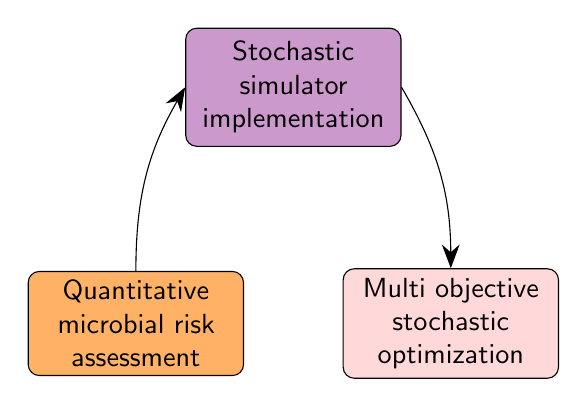
\begin{tikzpicture}[
	block1/.style={rectangle, rounded corners, draw, text width=2.5cm, minimum height=1cm, align=center, fill=orange!60},
        block2/.style={rectangle, rounded corners, draw, text width=2.5cm, minimum height=1cm, align=center, fill=pink!60},
        cheese/.style={rectangle, rounded corners, draw, text width=2.5cm, minimum height=1.5cm, align=center, fill=violet!40},
    arrow/.style={-{Stealth[length=3mm]}, bend angle=45, bend left=15},
    blank/.style={}
    ]
  
    % Blocks
    \node[block1] (qra) at (-2, 0) {Quantitative microbial risk\\ assessment};
    \node[block2] (moso) at (2, 0) {Multi objective\\stochastic optimization};
    \node[cheese] (sim) at (0, 3) {Stochastic\\simulator \\ implementation};
    
    % Cheese
%	\node[inner sep=0pt] (cheese) at (0, 1.5) {\includegraphics[width=2cm]{figures/camembert.png}};
    
    % Arrows
    \draw[arrow] (qra.north) to (sim.west);
    \draw[arrow] (sim.east) to (moso.north);
 

\end{tikzpicture}
\end{adjustbox}
\caption{Proposed workflow in the context of this thesis.}
\label{fig:elements}
\end{figure}
\newpage 
%-----------------------------------------------------------------------

%-----------------------------------------------------------------------
%	TABLE OF CONTENTS
%-----------------------------------------------------------------------

%\thispagestyle{empty} % No slide header and footer

\tableofcontents
\clearpage 
% -----------------------------------------------------------------------
\addtocounter{page}{-1} 
\vspace{30cm}
\begin{center}
	\Large{\textbf{Chapter 1}}
	\par
	\vspace{0.5cm}
	\large{\textbf{QMRA - Quantitative Microbial Risk Assessment}}
\end{center}
\begin{figure}[H]
  	\centering
		\includegraphics[width=0.3\textwidth]{images/camembert.png}
	\end{figure}
\vspace{-5cm}
\clearpage
% ----------------------------------------------------------------------
\section{Quantitative Microbial Risk Assessment}
\normalsize
\begin{itemize}
	\item \myred{What is QMRA ?}
		\tcbox{exposure to microbial pathogens} $\rightarrow$
		\tcbox{risk of illness}
	\item \myblue{QMRA literature for raw milk cheese}
	\begin{itemize}
		\item[]1. Pathogenic (MPS) STEC $-$ 
			\mybrown{\cite{perrin14}, $\hdots$}
		\item[]2. \textit{Salmonella} $-$ \mybrown{\cite{fares07, 
			teunis10}, $\hdots$}
		\item[]3. \textit{Listeria mono.} $-$ 
			\mybrown{\cite{sanaa04, efsa18}, $\hdots$}
	\end{itemize}
	\item \myblue{ArtiSaneFood objectives}
	\begin{itemize}
		\item Propose the \myred{first multipathogen QMRA model} 
			for raw milk cheese
		\item Use QMRA model to \myred{optimize intervention} steps 
	\end{itemize}
\end{itemize}

\clearpage
% ----------------------------------------------------------------------
\subsection{How to build a QMRA model?}
\begin{itemize}
	\item Framework established by \mybrown{\cite{codex99}}
\end{itemize}
\vspace{-0.5cm}
\begin{figure}[H]
  	\centering
		\includegraphics[width=\textwidth]{images/QMRA/farm2fork_perrin.pdf}
		\caption{Raw milk cheese \myred{Farm-to-Fork} QMRA
		model by \mybrown{\cite{perrin14}}}
	\end{figure}
\newpage
% ----------------------------------------------------------------------
\subsection{Extension to multipathogen framework}
\begin{itemize}
	\item \myblue{Production of one batch of cheese} - 
		\myred{$20,000 - 25,000$ cheeses}
\end{itemize}
\vspace{-0.5cm}
\begin{figure}[H]
  	\centering
		\includegraphics[width=\textwidth]{images/QMRA/farm2fork.pdf}
		\caption{Multipathogen \myred{Farm-to-Fork} 
		model by \mybrown{\cite{basakicpmf23}}}
	\end{figure}
\newpage
% ----------------------------------------------------------------------

\subsection{Farm module - milk contamination}
%\begin{itemize}
	\begin{itemize}
		\item \tcbox{Direct approach} \textit{Listeria 
			monocytogenes}
			$$
			Y_{\rm Lm}^{\rm milk} \sim 
			\mypurple{\lognormal} 
			\text{ \mybrown{\citep{sanaa04}}}
			$$ 
		\item \tcbox{Indirect approach} STEC and 
			\textit{Salmonella} 
		\begin{align*}
			Y_{\rm pathogen}^{\rm milk} = 
			Y_{\rm Ecoli}^{\rm milk} 
			\cdot 
			\left( Y^{\rm feces}_{\rm pathogen}/
			Y^{\rm feces}_{\rm Ecoli} \right)
		\end{align*}
		%\vspace{3mm}
		\begin{itemize}
			\item []$\rightarrow$ \myred{Why ?} Limit of 
				detection due to low concentration 
			\item[]$\rightarrow$ \myred{How ?} Using
				concentration in animal feces 
				$Y^{\rm feces}_{\rm pathogen}$ and 
				$Y_{\rm Ecoli}^{\rm milk}$
			\item[]$\rightarrow$ \myred{Parameters ?} 
				\mybrown{\cite{perrin14, bonifait21}}

				%$$Y^{\rm feces}_{\rm Salmo},\  
				%Y^{\rm feces}_{\rm Ecoli} \sim 
				%\mypurple{\lognormal}, 
			        %Y_{\rm STEC}^{\rm feces} \sim 
				%\mypurple{\weibull}$$%
		\end{itemize}	

	\item \myblue{Outputs}: Simulated pathogen concentration in milk
	\end{itemize} 
\newpage 
%-----------------------------------------------------------------------
\subsection{Cheese module - pathogen evolution}
\normalsize
\begin{itemize}
	\item \myblue{Growth $\nearrow$ phase} 
	\begin{itemize}
		\item Logistic model with rate 
			\myred{$\mu_x(\text{Temp.}, \text{pH}, \hdots)$} \mybrown{\citep{augustin2005}}
	\end{itemize}
\end{itemize}
%\vspace{-0.4cm}
%\begin{align*}
%	\frac{dy}{dt} = \myred{\mu^{\rm max}_{x}}(t) \cdot y(t) \cdot 
%	(1-\frac{y(t)}{y^{\rm max}})
%\end{align*}
\tcbox{Milk storage} $\rightarrow$ \tcbox{Molding} $\rightarrow$ \textit{Colony formation} 
$\rightarrow$ \tcbox{Draining} $\rightarrow$ \tcbox{Salting}
\begin{itemize}
	\item \myblue{Decline $\searrow$ phase} 
	\begin{itemize}
		\item Decline rates \myred{$\rho_x$} \mybrown{\citep{perrin14, barron22}}
	\end{itemize}
\end{itemize}
%\vspace{-0.4cm}
	%\begin{align*}
	%\myred{\text{STEC}} &: Y_{\rm STEC}(t) = Y^{\rm salting}_{\rm STEC}
	%\cdot 10^{-\rho \cdot t} \\
	%\myred{\textit{\text{Salmonella}}} &: Y_{\rm Salmo}(t) = Y^{\rm 
	%salting}_{\rm Salmo} \cdot 10^{-(t/\delta)^p} 
	%\end{align*}
\begin{center}
	\tcbox{Ripening} $\rightarrow$ \tcbox{Cheese storage} $\rightarrow$ \tcbox{Consumption}
%\begin{align*}
	%\myred{\textit{\text{Listeria}}} &: Y^{\rm end.salting}_{\rm Lm} = 
	%Y^{\rm salting}_{\rm Lm} \cdot 10^{-\rho_{\rm Lm}} + 
	%\end{align*}
\end{center}
\begin{itemize}
	\scriptsize
	\item[] N.B. \myblue{\text{Second\ growth\ 
		$\nearrow$ phase}}: After Salting for \textit{Listeria}
	\normalsize
	\item \myblue{Outputs}: Simulated \myred{number} 
		$N_x^{\rm colony}$ and \myred{size} of colonies for 
		\myred{pathogen $x$}
\end{itemize}
\clearpage
% -----------------------------------------------------------------------
\subsection{Consumer module - risk estimation}
\normalsize
\begin{itemize}
	\item \myblue{Dose in $1$ cheese serving} $\Gamma_x = $ (Number 
		$\times$ size) of colonies$_x$
	\item \myblue{Risk from $1$ cheese serving} - \myred{Dose-response 
		model}		
\begin{align*}
	P^{\rm illness}_{\rm STEC}(\text{Age}, \Gamma_{\rm STEC}) \rightarrow \text{\mybrown{\cite{perrin14}}} \\
	P^{\rm illness}_{\rm Salmo}(\Gamma_{\rm Salmo}) \rightarrow \text{\mybrown{\cite{strickland23}}} \\ 
	P^{\rm illness}_{\rm Listeria}(\text{Age}, \Gamma_{\rm Lm}) \rightarrow \text{\mybrown{\cite{efsa18}}} 
\end{align*}
	\item \myblue{Risk of illness conditional on} \myred{batch 
		characteristics} \mygreen{$\Xi_x = \xi_x$} 
\begin{align*}
	R^{\rm batch}_{x}(\mygreen{\xi_x}) = \sum_{\myred{\rm{age}}}
	g({\myred{\rm{age}}}) \cdot 
	\Esp_{\Gamma_{x}}[P^{\rm illness}_{x}(\myred{\text{age}}, 
	\Gamma_x) \mid \mygreen{\Xi_x = \xi_x}]
\end{align*}
	\scriptsize
	\item[]$\rightarrow g(\myred{\rm{age}})$: proportion of cheese 
		consumption per age group
	\item[]$\rightarrow \mygreen{\Xi_x}$: stochastic internal 
		variables simulated by the QMRA model
\end{itemize}
\clearpage
% -----------------------------------------------------------------------
\subsection{How to reduce pathogen contamination?}
\begin{itemize}
	\item \myblue{Intervention steps} - \myred{food safety regulations}
\end{itemize}
\vspace{-0.5cm}
\begin{figure}[H]
        \centering
                \includegraphics[width=\textwidth]{images/QMRA/farm2fork_interv.pdf}
		\caption{Implementation of \myblue{pre-harvest} and 
		\myblue{post-harvest} intervention steps}
        \end{figure}
\newpage
% ----------------------------------------------------------------------
\subsection{Intervention - reduce contamination}
\begin{itemize}
	\item \tcbox{Pre-harvest} \myblue{Testing farm milk} with frequency 		\myred{$p_{\rm milk}$}
	\begin{itemize}	
		\item Rejecting farms with high \textit{E. coli} 
			contamination in milk
	\begin{align*}
		Y_{\rm Ecoli}^{\rm milk} > \myred{l_{\rm milk}}\ \ {\rm CFU}
	\end{align*}
	\end{itemize}
	\item \tcbox{Post-harvest} \myblue{Testing cheese batch} with 
		frequency \myred{$p_{\rm cheese}$}
	\begin{itemize}
		\item P[at least one tested samples is contaminated by 
			pathogen $x$]
	\begin{align*}
		P^{\rm reject}_x(\Xi_x) = 1 - (1 - 
		P[N_x^{\rm colony} > 0])^{\myred{n_{\rm sample}}}
        \end{align*}
		\item Cheese batch is rejected if contaminated by 
			any pathogen $x$
	\end{itemize}
\end{itemize}
\newpage 
%-----------------------------------------------------------------------
\subsection{Outputs of QMRA model}
\normalsize
\begin{itemize}
	\item \myblue{One random simulated cheese batch} conditional on 
		$\Xi = (\Xi_x)_x$
	\begin{itemize}
		\item[]1. Batch risk \myred{$R^{\rm batch}_{x}(\Xi_x)$} 
			%(pathogen $x$)
		\item[]2. Amount of Milk rejected 
			\myred{$M^{\rm batch}$} %(in liters) 
		\item[]3. Prob. of rejecting a cheese batch 
			\myred{$P^{\rm batch}(\Xi)$}
	\end{itemize}
	\item \myblue{Average outputs for a cheese producer}
	\small
	\begin{itemize}	
		\item[]$1.$ 
		\myred{Average risk} (pathogen $x$) \\
		$$\myblue{R_{x}} = \frac{\mathbb{E}[R^{\rm 
		batch}_{x}(\Xi_x) 
		\cdot (1-P^{\rm batch}(\Xi)\cdot 
		p_{\rm cheese})]}{\mathbb{E}[1-P^{\rm batch}(\Xi) 
		\cdot p_{\rm cheese}]}$$
		\item[]$2.$ 
		\myred{Average cost}
		$$
		\myblue{C} = c_1 + c_2 \cdot \Esp[M^{\rm batch}] + 
		c_3 \cdot \Esp[P^{\rm batch}(\Xi) \cdot 
		p_{\rm cheese}],\ (c_i\text{'s} = \text{cost})
		$$
	\end{itemize}
	%\item[]$\rightarrow$ $c_i$'s denote cost values 
	%	\textit{\mybrown{(COPIL ArtiSaneFood, Caen, Normandie, 2022)}}
\end{itemize}
\clearpage
% ----------------------------------------------------------------------
\subsection{Multi-risk QMRA model for 3 pathogens}
\normalsize
\vspace{-1.2cm}
\begin{figure}[H]
  	\centering
		\includegraphics[width=0.85\textwidth]{images/QMRA/qmra_2.pdf}
\end{figure}
\vspace{-0.7cm}
\begin{itemize}
	\item \myblue{Model validation}: Compare risk/prevalence with
		previous studies
	\item \myblue{Aim}: Find \myred{optimal inputs} that minimize all 
		the outputs

\end{itemize}

\newpage
% ----------------------------------------------------------------------
\subsection{How to minimize 3 risks simultaneously?}
\normalsize
\vspace{-1.2cm}
\begin{figure}[H]
  	\centering
		\includegraphics[width=0.85\textwidth]{images/QMRA/qmra_3.pdf}
\end{figure}
\vspace{-0.7cm}
\begin{itemize}
	\item Different pathogens have \myred{different impact} on public 
		health
\end{itemize}
\newpage
% ----------------------------------------------------------------------
\subsection{DALY: Disability Adjusted Life Years}
\begin{itemize}
	%\item \myblue{Aim}: Evaluate the collective impact of all pathogens
	\item DALY = YLL (Years Lost) + YLD (Years with Disability)
	\item \myblue{Metric}: Average DALY from consuming a cheese 
		portion contaminated by pathogen $x$ from a batch that
		was not rejected
	\begin{align*}
		\overline{\text{DALY}}_{\text{portion}, x} = 
		\sum_{\myred{\text{age}}}
    		\overline{\text{DALY}}^{\rm portion}_{\text{illness}(x)}
		(\myred{\text{age}}) \cdot R_x(\myred{\text{age}}) \cdot 
		g(\myred{\text{age}})
	\end{align*}
	\item \myblue{Problem}: Lack of epidemiological studies to 
		estimate $\overline{\text{DALY}}^{\rm portion}_{
			\text{illness}(x)}(\myred{\text{age}})$
	\item \myblue{Simplified formulation}:
	\begin{align*}
		\overline{\text{DALY}}_{\text{portion}, x} =
		R_x \cdot \myred{\text{DALY(1 case)}_{x}}
	\end{align*}
	\small
	\begin{itemize}
		\item \myred{$\text{DALY(1 case)}_{x}$}: DALY for $1$ case
			of illness($x$) \mybrown{\citep{cassini18}}
	\end{itemize}
\end{itemize}
\newpage
% ----------------------------------------------------------------------
\subsection{Multipathogen risks measured in life years}
\vspace{-1.2cm}
\begin{figure}[H]
  	\centering
		\includegraphics[width=0.85\textwidth]{images/QMRA/daly_1.pdf}
\end{figure}
\vspace{-0.7cm}
\begin{itemize}
	\item \myred{Combined DALY} per portion 
	$\overline{\text{DALY}}_{\text{portion}} = \sum_x 
	\overline{\text{DALY}}_{\text{portion}, x}$
\end{itemize}
\newpage
% ----------------------------------------------------------------------
\subsection{Shall we aggregate again ?}
\vspace{-1.2cm}
\begin{figure}[H]
  	\centering
		\includegraphics[width=0.85\textwidth]{images/QMRA/final_qmra.pdf}
\end{figure}
\vspace{-0.7cm}
\begin{itemize}
	\item \myred{$\overline{\text{DALY}}_{\text{portion}}$} and 
		\myred{cost} are measured in different units!
\end{itemize}
\newpage
% ----------------------------------------------------------------------
\subsection{How to choose optimal intervention parameters?}
\begin{itemize}
    \item Consider discrete input space:
    \begin{itemize}
        \item \myblue{Prop. of cheese batches tested} 
	\myred{$p_{\rm cheese}$} : $\{10\%,\ 30\%,\ 50\%\}$
        \item \myblue{Number of samples} \myred{$n_{\rm sample}$} : 
            $\{1,\ 5,\ 10,\ 15\}$
        \item \myblue{Prop. of milk batches tested} 
		\myred{$p_{\rm milk}$} : $\{10\%,\ 50\%,\ 100\%\}$
	\item \myblue{Milk testing limit} \myred{$l_{\rm milk}$} (CFU/ml): 
            $\{10,\ 20,\ 30,\ 50,\ 100,\ 200\}$
    \end{itemize}
    \item Construct a \myred{scenario} $\rightarrow 
	    \{p_{\rm cheese},\ n_{\rm sample},\ p_{\rm milk},\ 
		l_{\rm milk}\}$
    \item Total possible scenarios: \myblue{$216$}
    \item $5000$ \myred{Monte Carlo} simulations on each scenario 
	    gives \tcbox{DALY} \& \tcbox{Cost}
\end{itemize}
\newpage 
% ----------------------------------------------------------------------
\begin{figure}[H]
	\centering
		\includegraphics[width=0.8\textwidth]{images/QMRA/post_3_pf.pdf}
\end{figure}
\newpage
% ----------------------------------------------------------------------
\subsection{Is cheese testing really effective?}
\begin{itemize}
	\item \tcbox{\textit{Listeria}} has a second growth $\nearrow$ 
		phase + unaffected by milk testing
	\item \myred{High prevalence} increases batch 
		rejection 
	\item \myblue{Lower risk} of getting \textit{Listeriosis} compared 
		to others pathogen illnesses
\end{itemize}
%\begin{figure}[H]
%	\centering
%	\includegraphics[width=0.4\textwidth]{images/QMRA/ecdf_p_reject.pdf}
%	\caption{ECDF for probability of batch detecction due to testing}
%\end{figure}
\begin{table}[H]
	%\caption{Baseline scenario (no intervention) average batch 
	%results} % 
\centering
\begin{adjustbox}{max width=\textwidth}
\begin{tabular}{c|c|c|c}
    \hline
	Metric & \textit{Listeria} & \textit{Salmonella} & MPS-STEC \\ 
    \hline 
	Average Prevalence ($\%$) & \myred{$39.47$} & $0.84$ & $1.97$ \\
	%$\Esp \left[ P^{\rm reject}_x(\Xi_x) \right]$ & \myred{$0.5$} & 
	%$0.1$ & $0.14$ \\
	$R_x / R_{\rm MPS-STEC}$ & \myblue{$\num{4.2e-5}$} & $0.1$ & $1$ \\
	$\overline{\text{DALY}}_{\text{portion}, x}/
	\overline{\text{DALY}}_{\text{portion}}$ & \myblue{$\num{4e-5}$} & 
	$\num{5e-4}$ & $0.99$ \\
    \hdashline
	$\text{DALY(1 case)}_{x}$ \mybrown{\citep{cassini18}} & $3.7$ & $0.019$ & $3.7$ \\
    \hline
\end{tabular}
\end{adjustbox}
\end{table}
\newpage 
% ----------------------------------------------------------------------
\subsection{Redefine cheese testing plan?}
\begin{itemize}
	\item $\text{DALY(1 case)}_{\rm Listeriosis} = \myred{3.7}$ years 
		\tcbox{BUT} Listeriosis has very \myred{low risk}!
	\item \myblue{Not all} \textit{Listeria} strains are highly 
		virulent ! \mybrown{\citep{pouillot24}}
	\item Rejection based on \myred{virulence} /  \myred{concentration}
		threshold?
\end{itemize}
\begin{table}[H]
	%\caption{Baseline scenario (no intervention) average batch 
	%results} % 
\centering
\begin{adjustbox}{max width=\textwidth}
\begin{tabular}{c|c|c|c}
    \hline
	Metric & \textit{Listeria} & \textit{Salmonella} & MPS-STEC \\ 
    \hline 
	Average Prevalence ($\%$) & \myred{$39.47$} & $0.84$ & $1.97$ \\
	%$\Esp \left[ P^{\rm reject}_x(\Xi_x) \right]$ & \myred{$0.5$} & 
	%$0.1$ & $0.14$ \\
	$R_x / R_{\rm MPS-STEC}$ & \myblue{$\num{4.2e-5}$} & $0.1$ & $1$ \\
	$\overline{\text{DALY}}_{\text{portion}, x}/
	\overline{\text{DALY}}_{\text{portion}}$ & \myblue{$\num{4e-5}$} & 
	$\num{5e-4}$ & $0.99$ \\
    \hdashline
	$\text{DALY(1 case)}_{x}$ \mybrown{\citep{cassini18}} & $3.7$ & $0.019$ & $3.7$ \\
    \hline
\end{tabular}
\end{adjustbox}
\end{table}

\newpage 
% ----------------------------------------------------------------------
\begin{figure}[H]
	\centering
		\includegraphics[width=0.8\textwidth]{images/QMRA/post_2_pf.pdf}
\end{figure}
\clearpage
% ----------------------------------------------------------------------
\begin{figure}[H]
	\centering
		\includegraphics[width=0.8\textwidth]{images/QMRA/pro.png}
\end{figure}
\clearpage
% ----------------------------------------------------------------------
\subsection{Key takeaways: chapter 1}
\begin{itemize}
	\item We propose the \myred{first multipathogen QMRA model} (raw 
		milk cheese)
	\begin{itemize}
		\item Risk assessment (DALY) + Cost estimation (€)
		\item \myblue{Conflicting objectives} -  
				\myred{several optimal scenarios}
		%\item Model based on \mybrown{\cite{perrin14, sanaa04}, 
		%	$\hdots$}
	\end{itemize}
	\item \myblue{Challenges}
		\begin{itemize}
			\item \myred{Noisy} - evaluations - 
			\myred{computationally expensive} 			    		    \item $4.5$ seconds $\times \, 5000$ batches 
				$\times \, 216$ scenarios $\approx 56$ days !!
		\end{itemize}
\end{itemize}
\begin{center}
		\Large
		\tcbox{How to find optimal scenarios using limited budget?}
\end{center}	
\newpage
% ----------------------------------------------------------------------
\addtocounter{page}{-1} 
\vspace{30cm}
\begin{center}
	\Large{\textbf{Chapter 2}}
	\par
	\vspace{0.5cm}
	\large{\textbf{MOSO - Multiobjective simulation optimization}}
\end{center}
\begin{figure}[H]
  	\centering
		\includegraphics[width=0.3\textwidth]{images/camembert.png}
	\end{figure}
\vspace{-5cm}
\clearpage
% ----------------------------------------------------------------------
\section{Multiobjective Simulation Optimization}
\vspace{-0.8cm}
\begin{figure}[H]
  	\centering
		\includegraphics[width=0.65\textwidth]{images/QMRA/pro.png}	
	%\caption{Outputs are averaged over batches}
\end{figure}
\clearpage
% ----------------------------------------------------------------------
\subsection{Identifying optimal scenarios by evaluating all points}
\vspace{-1cm}
\begin{figure}[H]
  	\centering
		\includegraphics[width=0.7\textwidth]{images/pf_2_pareto.pdf}
	%\caption{Outputs are averaged over batches}
\end{figure}
\newpage
% ----------------------------------------------------------------------
\subsection{First step: problem formulation}
\normalsize
\begin{itemize}
	\item Consider a multiobjective minimization problem of $f = (f_1, f_2,
		\hdots, f_q)$ 
	\begin{equation}
		\min_{x \in \mathbb{X}}f(x)
	\end{equation}
	\item \myblue{Noisy observations}: $Z^i_j = f_j(x^i) + 
		\varepsilon^i_j$, with noise 
		$\varepsilon^i_j \sim \mathcal{N}(0, {\tau^i_j}^2)$
	\item \myblue{Conflicting objectives}: No unique optimal solution
	\item The solution set consists of \myred{Pareto optimal} points 
	\begin{equation}
		\mathcal{P} = \{x\in \mathbb{X} : \nexists x^{\prime} \in \mathbb{X},
		f(x^{\prime}) \prec f(x)\}
	\end{equation}
	\item $f(x^{\prime}) \prec f(x) \implies f_j(x^{\prime}) \leq 
		f_j(x), \forall j$, with at least one strict inequality
\end{itemize}
\clearpage 
% -----------------------------------------------------------------------
\subsection{What is Pareto optimality?}
\large
\begin{center}
	\includegraphics[width=0.6\textwidth]{images/pareto_front_noise.pdf}
\end{center}
\normalsize
\begin{itemize}
	\item \myblue{Goal}:  Estimate the \emph{Pareto set} 
		\myred{$\mathcal{P}$} and \emph{Pareto front} 
		\myred{$\mathcal{F}$} (image of $\mathcal{P}$) 
	\item \tcbox{Main challenge} $\rightarrow$ \myred{Limited budget} + 
		\myred{noisy observations}
\end{itemize}
\clearpage
% ----------------------------------------------------------------------
\subsection{Surrogate models - Gaussian Process (GP) regression}
\vspace{-0.6cm}
%\begin{center}
%	\includegraphics[width=0.5\textwidth]{images/gpr.pdf}
%\end{center}
\begin{figure}[H]
\centering
\begin{subfigure}{.5\textwidth}
  \centering
  \includegraphics[width=0.93\linewidth]{images/gpr_1.pdf}
	%\caption{Function approximation \\ Sampling at \myred{maximal posterior variance}}
  \label{fig:sub1}
\end{subfigure}%
\begin{subfigure}{.5\textwidth}
  \centering
  \includegraphics[width=0.93\linewidth]{images/gpr.pdf}
	%\caption{Estimation of probability of failure \\ Sampling at \myred{maximal misclassification prob.}}
  \label{fig:sub2}
\end{subfigure}
\label{fig:mus_demo}
\end{figure}
\vspace{-0.6cm}
\begin{equation}
	Z^i_j = \xi_{j}(x^i) + \varepsilon^i_j \text{ with } 
	\varepsilon^i_j \overset{\text{ind.}}{\sim} 
	\mathcal{N}(0, \tau_j^2),\quad i=1, 2, \hdots
\end{equation}
%\vspace{0.01cm}
\begin{itemize}
	\item $\xi_j$s are independent GPs with mean 
		$m_j$ and covariance $k_j$, $j=1,\ldots,\,q$
	\item \myred{Posteriors} of $\xi_j \mid Z^i_j$ are computed by 
		solving system of linear equations 
		%\mybrown{\citep{rasmussen06}}
\end{itemize}
\clearpage
% ----------------------------------------------------------------------
\subsection{How to use GP regression in optimization?}
\begin{algorithm}
\caption{Bayesian Optimization (BO)}
\label{alg:bo}
\begin{algorithmic}
%\State Place Gaussian process prior on $f$ \Comment{(surrogate model)}
	\State \mybrown{Sample}\myred{$^{\ast}$} $f$ at $n_0$ points %\Comment{(initial design)}
%\State $n \gets n_0$ and $b \gets n_0 \times k$ 
	\While{\myred{budget} $> 0$} 
	\State \myblue{Update} : GP posterior $\xi \mid Z^1, Z^2, \hdots, 
	Z^n$
	\State \myblue{Compute} : \emph{\mygreen{acquisition function}} $J_n(x)$
	\State \myblue{Optimize} : $x_{n+1} = \argmax_{x \in \mathbb{X}}J_n(x)$ %\Comment{(new observation)}
	\State \myblue{Sample}\myred{$^{\ast}$} : $f$ at $x_{n+1}$ 
%	\State $n \gets n+1$ and $b \gets b+k$	\Comment{(increment budget)}
\EndWhile
	\State Estimate\myred{$^{\ast\ast}$} $\hat{\mathcal{P}}$ and $\hat{\mathcal{F}}$ 
\end{algorithmic}
\end{algorithm}
\small
\myred{$\ast$} $f$ is sampled with a batch size $k$
\newline
\myred{$\ast\ast$} $\hat{\mathcal{P}}$ and $\hat{\mathcal{F}}$ are estimated with GP posterior mean $\mu_n(x)$
\clearpage
% ----------------------------------------------------------------------
\subsection{How to construct an acquisition function $J(x)$?}
\normalsize
\begin{figure}[H]
\centering
\begin{adjustbox}{max width=0.8\textwidth}
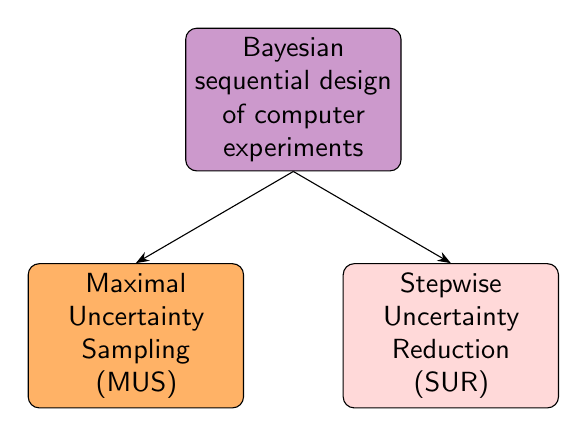
\begin{tikzpicture}[
	block1/.style={rectangle, rounded corners, draw, text width=2.5cm, minimum height=1cm, align=center, fill=orange!60},
        block2/.style={rectangle, rounded corners, draw, text width=2.5cm, minimum height=1cm, align=center, fill=pink!60},
        cheese/.style={rectangle, rounded corners, draw, text width=2.5cm, minimum height=1.5cm, align=center, fill=violet!40},
    arrow/.style={-{Stealth[length=3mm]}, bend angle=45, bend left=15},
    blank/.style={}
    ]
  
    % Blocks
	\node[block1] (mus) at (-2, 0) {Maximal Uncertainty Sampling \\ 
	(MUS)};
	\node[block2] (sur) at (2, 0) {Stepwise Uncertainty Reduction 
	\\ (SUR)};
    	\node[cheese] (dace) at (0, 3) {Bayesian sequential design of 
	computer experiments};
    
    % Cheese
%	\node[inner sep=0pt] (cheese) at (0, 1.5) {\includegraphics[width=2cm]{figures/camembert.png}};
    
    % Arrows
    \draw[-Stealth] (dace.south) -- (mus.north);
    \draw[-Stealth] (dace.south) -- (sur.north);
 

\end{tikzpicture}
\end{adjustbox}
%\caption{Proposed workflow in the context of this thesis.}
%\label{fig:elements}
\end{figure}
% ----------------------------------------------------------------------
\subsection{How to assess performance of a BO algorithm?}
\vspace{-0.2cm}
\begin{itemize}
	\item[]1. \tcbox{Volume of Symmetric Difference (VSD)} on 
		\myred{Pareto front} $\mathcal{F}$ 
		%(image of $\mathcal{P}$)
	%\begin{itemize}
	%	\item[]$\rightarrow$ Uses dominated region between $\mathcal{F}$ and a reference point $R$
	%\end{itemize}
\end{itemize}
\vspace{-0.5cm}
\begin{figure}[H]
  	\centering
	\includegraphics[width=0.9\textwidth]{images/VSD_demo.pdf}
	\caption{\myred{True} Pareto front, \myblue{Estimated} Pareto front
		and reference $R$}
\end{figure}
\begin{itemize}
	\item[]2. \tcbox{Misclassification Rate (MCR)} on \myred{Pareto set} 
		$\mathcal{P}$
\end{itemize}
\clearpage
% ----------------------------------------------------------------------
\subsection{Maximal uncertainty sampling}
%\vspace{-3mm}
\begin{itemize}
	\item \myblue{Idea} : Sample at $x \in \mathbb{X}$ where 
		\myred{uncertainty} is maximum
	\item Application in different design of experiment frameworks:
\vspace{-3mm}
\begin{figure}[H]
\centering
\begin{subfigure}{.5\textwidth}
  \centering
  \includegraphics[width=0.93\linewidth]{images/func_approx.pdf}
	\caption{Function approximation \\ Sampling at \myred{maximal posterior variance}}
  \label{fig:sub1}
\end{subfigure}%
\begin{subfigure}{.5\textwidth}
  \centering
  \includegraphics[width=0.93\linewidth]{images/excursion.pdf}
	\caption{Estimation of probability of failure \\ Sampling at \myred{maximal misclassification prob.}}
  \label{fig:sub2}
\end{subfigure}
\label{fig:mus_demo}
\end{figure}
\end{itemize}
\clearpage
% ----------------------------------------------------------------------
\subsection{A first idea with MUS}
\vspace{-0.3cm}
\begin{itemize}
	\item Sampling at maximal probability of misclassification 
		\mybrown{\citep{bryan05}}
	\item $J_n(x)$: \myred{Bernoulli variance} of the indicator function $\mathbb{1}_{\{x \in \mathcal{P}\}}$
	\begin{align*}
		\Var_n{(\mathbb{1}_{\{x \in \mathcal{P}\}})} = p_n(x) \cdot (1-p_n(x))
	\end{align*}
	%\begin{itemize}
	$\rightarrow$ Estimated with \myblue{conditional simulations} of 
			$\xi_n$ \mybrown{\citep{binois15}}
	%\end{itemize}
	\vspace{-0.3cm}
	\begin{figure}[H]
  	\centering
	\includegraphics[width=0.37\textwidth]{images/misclassification.pdf}
	\vspace{-0.3cm}
		\caption{Equivalent measures in literature 
		\mybrown{\citep{bect11}}}
	\label{fig:mus_fail}
\end{figure}
\vspace{-0.3cm}
\end{itemize}
\clearpage
% ----------------------------------------------------------------------
\subsubsection{Performance on test problem g1 from \cite{barracosa21}}
\begin{figure}[h]
\centering
\begin{subfigure}{.5\textwidth}
  \centering
  \includegraphics[width=0.85\linewidth]{images/svd_mean_g1_fail.pdf}
  \caption{Vol. of symm. difference}
  \label{fig:sub1}
\end{subfigure}%
\begin{subfigure}{.5\textwidth}
  \centering
  \includegraphics[width=0.85\linewidth]{images/mcl_mean_g1_fail.pdf}
  \caption{Misclassification rate}
  \label{fig:sub2}
\end{subfigure}
	\caption{\small Average performance of \myred{$p_n \cdot (1-p_n)$} 
	based MUS method compared to a naive \myyellow{Random Search} (RS) 
	baseline method that samples $X_{n+1}$ randomly from $\mathbb{X}$}
\label{fig:test}
\end{figure}
\begin{center}
\normalsize
	\myred{This method does not work!!}
\end{center}
\clearpage
% ----------------------------------------------------------------------
\subsubsection{Why it fails ?}
\normalsize
\vspace{-0.5cm}
\begin{figure}[H]
  	\centering
	\includegraphics[width=0.85\textwidth]{images/mus_fail.pdf}
	\caption{Zoomed from left figure on right, with $p_n(x)$ and 
	post. uncertainty}
	\label{fig:mus_fail}
\end{figure}
\begin{itemize}
	\item \myred{Red point} $p_n(x) \approx 0.5 \rightarrow$ 
		\tcbox{difficult to classify} $\rightarrow$ due to its 
		\myblue{neighbors}
	\item The algorithm gets \myred{stuck} at such points and 
		samples \myred{repetitively}
	\item Reducing their post. uncertainty not improving the 
		acquisition criterion
\end{itemize}
\clearpage
% ----------------------------------------------------------------------
\subsection{Weighted Mean Squared Error (w-MSE)}
\normalsize
\begin{itemize}
	\item \myblue{Not all uncertainty measures can be reduced by MUS!}
	\item We try to reduce the \myred{weighted mean squared error}
	\begin{align*}
		\centering
		X_{n+1} = \argmax_{x \in \mathbb{X}} \bigg( w_n(x) \cdot 
		\sum_{j=1}^q
		\frac{\sigma_{j, n}^2(x)}{R^2_{j, n}} \bigg) 
	\end{align*}
	$R_{j, n}$ is a normalizing constant for $j = 1, 2, \hdots, q$ -th objective
	\item \myblue{Weights} \tcbox{$w_n(x)$} target the 
		``\myred{potential Pareto optimal}'' region 	
	\item \myblue{Choice of weights ?} 
	\begin{itemize}
		\item We proposed $w_n(x)$ based on \myred{$p_n(x)$} (see 
			Appendix~\ref{app3}) 
		\item $0$ - $1$ weights $\rightarrow$ \myred{PAL} 
			algorithm \mybrown{\citep{zuluaga13}}
	\end{itemize}
\end{itemize}
\clearpage
% ----------------------------------------------------------------------
\subsection{PALS (PAL + stochastic setting): \cite{barracosa21}}
\normalsize
%\vspace{-0.3cm}
\begin{itemize}
	\item PALS is a \myblue{w-MSE} algorithm with \tcbox{$w_n(x) = 
		\mathbb{1}_{\{x \in \mathbb{X} \setminus N_n\}}$}
	%\vspace{0.2cm}
	%\begin{align*}
	%	N_n  = \{x \in \mathbb{X}|\exists x^{\prime}
	%        \in \mathbb{X} \setminus \{x\}, R^{+}_n(x^{\prime})
	%        \prec R^{-}_n(x)\}
	%\end{align*}	
\end{itemize}
\vspace{-0.5cm}
\begin{figure}[H]
\centering
\begin{subfigure}{.55\textwidth}
  \centering
  \includegraphics[width=0.9\linewidth]{images/pals.pdf}
\caption{\myblue{Confidence rectangle}}
  \label{fig:pals_rect}
\end{subfigure}%
\begin{subfigure}{.45\textwidth}
  \centering
  \includegraphics[width=0.7\linewidth]{images/classify_n.pdf}
	\caption{\mygreen{$R_n^{+}(x^{\prime})$} $\prec$ \myred{$R_n^{-}(x)$}}
  \label{fig:sub2}
\end{subfigure}
\label{fig:pals}
\end{figure}
\vspace{-0.5cm}
\begin{itemize}
	\item $x\in N_n$ if \myred{optimistic $R_n^{-}(x)$} is dominated by some 
		\mygreen{pessimistic $R_n^{+}(x^{\prime})$} 
\end{itemize}
\clearpage
% ----------------------------------------------------------------------
\subsubsection{w-MSE methods against PALS (\myred{No consistent improvement})}
\begin{figure}[h]
\centering
\begin{subfigure}{.5\textwidth}
  \centering
  \includegraphics[width=0.8\linewidth]{images/w-MSE/mean/svd_mean_g1_mse.pdf}
  \caption{VSD on g1}
  \label{fig:sub1}
\end{subfigure}%
\begin{subfigure}{.5\textwidth}
  \centering
  \includegraphics[width=0.8\linewidth]{images/w-MSE/mean/svd_mean_g2_mse.pdf}
  \caption{VSD on g2}
  \label{fig:sub2}
\end{subfigure}
\caption{\small Average performance of \myblue{PALS} with \mygray{w-MSE} methods and \myyellow{Random Search}}
\label{fig:test}
\end{figure}
\begin{center}
\normalsize
	PALS being a \myred{simple} and \myred{inexpensive} 
	algorithm \\
	\myblue{remains difficult to beat in MUS framework!!}
\end{center}
\clearpage
% ----------------------------------------------------------------------
\subsection{Stepwise uncertainty reduction?}
\normalsize
\begin{itemize}
	\item \myblue{Origins \& applications} : reliability theory, optimization, $\hdots$
		\begin{itemize}
			\item \mybrown{\cite{vazquez06}, 
				\cite{villemonteix07}, 
				\\ \cite{vazquez09}}, $\hdots$
		\end{itemize}
	\item \myblue{Quantification of uncertainty at step} $n$$ : H_n$ 
	\begin{itemize}
		\item Acquisition function is \myred{minimized} to sample 
			$X_{n+1}$
		\begin{align*}
			J_n(x) = \mathbb{E}_n(H_{n+1}|X_{n+1}=x)
		\end{align*}
		\item $\mathbb{E}_n$ : conditional expectation w.r.t $\{X_1, Z_1, \hdots, 
			X_n, Z_n\}$
		\item \myred{$J_n(x)$ does not always have a closed 
			analytical form}
	\end{itemize}
\end{itemize}
\clearpage
% ----------------------------------------------------------------------
\subsection{Weighted Integrated Mean Squared Error (w-IMSE)}
\begin{itemize}
	\item \myblue{w-IMSE} as uncertainty measure $H_n$ gives the 
		following acquisition
	\begin{align*}
		X_{n+1} = \argmin_{x \in \mathbb{X}}\sum_{i=1}^{\abs{\mathbb{X}}} w_n(x_i)
		\sum_{j=1}^q\frac{\sigma_{j, n+1}^2(x_i | x)}{R^2_{j, n}}
	\end{align*}
	\begin{center}
		\myred{How to choose a good weight $w_n(x)$ function?}
	\end{center}
	\item SUR criterion when $w_n(x_i) = p_n(x_i)$ 
	\item Other choice of ``\myred{plug-in}'' weights
	\begin{itemize}
		\item \myblue{PALS} based : $w_n(x_i) = \mathbb{1}_{\{x_i \in \mathbb{X} \setminus N_n\}} $
	%\item Based on uncertainty measures on \myblue{$\mathcal{F}$} 
	%	\mybrown{\citep[see, e.g.,][]{binois_thesis}}
		\item \myblue{Proposed weights} : \myred{PALS} 
			classification + deviations of \myred{$\mathcal{F}$}
	\end{itemize}
\end{itemize}
\clearpage
% ----------------------------------------------------------------------
\normalsize{\textbf{Proposed weights - focused on the VSD metric}}
\begin{figure}[H]
  	\centering
	\includegraphics[width=0.9\textwidth]{images/VSD_weight.pdf}
	\caption{Pareto front \myblue{$\hat{\mathcal{F}}$}, \myred{$\hat{\mathcal{F}_p}$} and 
	\mygreen{$\hat{\mathcal{F}_o}$} with dominated volumes \myred{$V_{n}$} 
	and \mygreen{$V_{n, i}$}}
\end{figure}
\begin{center}
$w_n(x_i) \leftarrow \mathbb{1}_{\{x_i \in \mathbb{X} \setminus N_n\}} \cdot 
(V_{n, i}-V_{n})$
\end{center}
\clearpage
% ----------------------------------------------------------------------
\normalsize
\begin{figure*}

\begin{center}
 \includegraphics[width=.4\linewidth]{images/w-IMSE/mean/svd_mean_g3.pdf} \hspace{5mm}
 \includegraphics[width=.4\linewidth]{images/w-IMSE/mean/svd_mean_g4.pdf} \\
 \vspace{0.1mm}

 \includegraphics[width=.4\linewidth]{images/w-IMSE/mean/svd_mean_g5.pdf}\hspace{5mm}
 \includegraphics[width=.4\linewidth]{images/w-IMSE/mean/svd_mean_g6.pdf}
	\caption{Average \myred{VSD metric} on problems g-3,4,5,6 
	\mybrown{\citep{barracosa21}}}

\end{center}
\end{figure*}
\clearpage
% ----------------------------------------------------------------------
\normalsize
\begin{figure*}

\begin{center}
 \includegraphics[width=.4\linewidth]{images/w-IMSE/mean/mcl_mean_g3.pdf} \hspace{5mm}
 \includegraphics[width=.4\linewidth]{images/w-IMSE/mean/mcl_mean_g4.pdf} \\
 \vspace{0.1mm}

 \includegraphics[width=.4\linewidth]{images/w-IMSE/mean/mcl_mean_g5.pdf}\hspace{5mm}
 \includegraphics[width=.4\linewidth]{images/w-IMSE/mean/mcl_mean_g6.pdf}
	\caption{Average \myred{MCR metric} on problems g-3,4,5,6 
	\mybrown{\citep{barracosa21}}}

\end{center}
\end{figure*}
\clearpage
% ----------------------------------------------------------------------
\subsection{Key takeaways: chapter 2}
\begin{itemize}
	\item Proposed w-IMSE method \myred{improves consistently over PALS}
	\begin{itemize}
		\item \mygreen{Improvement the VSD metric} on 
			$\mathcal{F}$ \mybrown{\citep{basakmascot23}} 
		\item \mygreen{Improvement on simulation budget} for a 
			given performance
	\end{itemize}
	\item \tcbox{However}: Difficult to beat PALS w.r.t both MCR and VSD
	\item \myblue{Remarks on PALS} 
	\begin{itemize}
		\item A \myred{simple}, \myred{inexpensive}, 
			\myred{easy-to-implement} MUS algorithm 
		\item Not easy to beat even with sophisticated SUR methods
	\end{itemize}
	\item \myblue{Application QMRA}: Proposed extension of PALS 
		\mybrown{\citep{basakmascot22}}
\end{itemize}
\clearpage
% -----------------------------------------------------------------------
\addtocounter{page}{-1} 
\vspace{30cm}
\begin{center}
	\large{\textbf{Contributions and perspectives}}
\end{center}
\begin{figure}[H]
  	\centering
		\includegraphics[width=0.3\textwidth]{images/camembert.png}
	\end{figure}
\vspace{-5cm}
\newpage
% ----------------------------------------------------------------------
\section{Contributions and perspectives}
\subsection{QMRA model development}
\begin{center}
	\tcbox{Ensuring food safety} + \tcbox{optimize analytical cost}
\end{center}
\begin{itemize}
	\item Proposed \myred{first multipathogen QMRA model} for raw milk 
		cheese
	\item ICPMF-12 Japan \mybrown{\citep{basakicpmf23}} + Article MRA 
		(under review)
	\item \myblue{Key features}:
	\begin{itemize}
		\item Assess burden on public health - \myred{DALY}s
		\item Estimation of \myred{intervention costs} 
		\item Parameter estimation with ArtiSaneFood 
			\myred{project data}
	\end{itemize}
\end{itemize}
\newpage
% ----------------------------------------------------------------------
\subsection{Article FESMJ + model FSKX \citep{basak23}}
\begin{figure}[H]
        \centering
                \includegraphics[width=0.9\textwidth]{images/conso/fskx.png}
	\caption{KNIME (\myred{open source GPLv3}) user interface for FSKX model}
\end{figure}
\newpage
% ----------------------------------------------------------------------
\subsection{Multipathogen model in R-shiny (WIP!)}
\begin{figure}[H]
        \centering
                \includegraphics[width=0.7\textwidth]{images/conso/actalia.png}
	\caption{R-shiny application for the \myred{cheese professionals}}
\end{figure}
\newpage
% ----------------------------------------------------------------------
\subsection{QMRA model in optimization}
\begin{itemize}
	\item ``Classical'' \myblue{scenario-based} analysis is common in 
		QMRA literature
	\item This becomes impractical with high simulation cost
        \begin{center}
                \tcbox{Novel approach}
        \end{center}	
	\item Optimization of \myred{multipathogen risk} and 
		\myred{intervention cost} simultaneously!
	\item \myblue{Approach}: Multiobjective simulation optimization 
		(MOSO) algorithms
	\item \myblue{Why MOSO algorithms?} 	
	\begin{itemize}
		\item Optimize \myred{expensive stochastic} simulator
		\item Estimate \myred{Pareto optimal} solutions in 
			\myred{limited budget}
		%\item We propose an extension of PALS algorithm  
		%	\mybrown{\citep{basakmascot22}}
	\end{itemize}	
\end{itemize}
\newpage
% ----------------------------------------------------------------------
\subsection{Multiobjective simulation optimization}
\begin{itemize}
	\item We study MUS and SUR based MOSO algorithms 
	\item Numerical benchmark against PALS algorithm 
	\item \myblue{Proposed a w-IMSE based pseudo-SUR algorithm}
		\mybrown{\citep{basakmascot23}}
	\begin{itemize}
		\item Weights based on the uncertainty on the Pareto front
			(\myred{$\mathcal{F}$})
		\item Significant \myred{improvement} over PALS on 
			estimation of $\mathcal{F}$
	\end{itemize}
	\item \myblue{Remarks on MUS principle based algorithms}
	\begin{itemize}
		\item Well-known sampling criteria from 
			\myred{reliability theory} literature are 
			inefficient in MOSO framework
		\item Not all uncertainty measures can be reduced by MUS!
	\end{itemize}
	
\end{itemize}
\newpage
% ----------------------------------------------------------------------
\subsection{QMRA perspectives} 
\myblue{Model calibration}: ``\textit{Models are always incomplete 
representations of the system they are intended to model, but they can 
still be useful.}'' \mybrown{\citep{who21}}
\begin{itemize}
		%\begin{itemize}
			%\item Lack of relevant data - expensive to collect
			%\item Model outputs compared with previous studies
		%\end{itemize}
	%\item \myblue{DALYs, Risks} should be \myred{interpreated 
	%	judiciously}!
	%\item \myblue{Computation of DALY} using relevant epidemiological 
	%	data
	\item[]1. \myblue{Farm module} for \textit{Listeria}
		\begin{itemize}
			\item \myred{Exposure assessment} is more difficult 
				than other pathogens
		\end{itemize}
	\item[]2. \myblue{Milk testing} step depends only on 
		\textit{E. coli} 
	\begin{itemize}
		\item Improve milk testing based on 
			\myred{\textit{Listeria} + \textit{Salmonella}} 
			detection? 
		\item Implement \myred{inclusion-exclusion} of farms + 
			dynamic hygiene parameters
	\end{itemize}
	\item[]3. \myblue{Cheese testing} for \textit{Listeria}
		%$\implies$ \myred{increases cost}
		%\vspace{-0.2cm}
		%\begin{center}
		%\tcbox{But} \\ 
		%\vspace{0.2cm}
		%\myred{No significant risk reduction!}
		%\end{center}
		%\vspace{-0.4cm}
	\begin{itemize}
		\item Redefine cheese testing considering 
			\myred{virulence} / \myred{threshold}?
	\end{itemize}
\end{itemize}
\newpage
% ----------------------------------------------------------------------
\subsection{MOSO perspectives}
\begin{itemize}
	%\item How to improve over PALS on the \emph{MCR metric}?
	%\begin{itemize}
	%	\item \myred{Tractable SUR} strategies over w-IMSE?
	%	\item w-IMSE with weights based on uncertainty on 
	%		$\mathcal{P}$?
	%\end{itemize}
	%\item How to improve over PALS on \emph{both MCR and VSD metric}?
	\item[]1. \myblue{QMRA applicability}: objective not 
		an expectation of simulator output
	\begin{itemize}
		\item Extended PALS \mybrown{\citep{basakmascot22}} 
			algorithm
		%\item $R_n^+, R_n^-$ replaced by empirical quantiles
		\item \myblue{Perspective}: similar extension for proposed
			w-IMSE algorithm 
		\item \myblue{Challenge}: Estimation of 
			$\sigma_{n+1}^2(x_i \mid x)$ inside w-IMSE 
			criterion 
		\item Use of Monte Carlo simulations from $\xi$ 
			(\myred{expensive})?
	\end{itemize}
	\item[]2. \myblue{Extension}: \myred{multiobjective} w-IMSE 
		algorithm + \myred{heteroscedastic} noise
	\item[]3. \myblue{Extend numerical benchmark}
	\begin{itemize}
		\item Ranking and selection \mybrown{\citep{lee10, rojas20}}
		\item Others \mybrown{\citep{belakaria2020, lobato14}}
	\end{itemize}
\end{itemize}
\newpage
% ----------------------------------------------------------------------
\Large
\begin{center}
	Thank you for your attention!
	\begin{figure}[H]
  	\centering
	\includegraphics[width=0.6\textwidth]{images/copil.jpg}
	\end{figure}
	\small
	\vspace{-0.5cm}
	COPIL ArtiSaneFood 2023, Maison du Lait, Paris
\end{center}
% -----------------------------------------------------------------------
\appendix
\addtocontents{toc}{\protect\setcounter{tocdepth}{0}}
% -----------------------------------------------------------------------
\clearpage
\addtocounter{page}{-1} 
\section{Appendix: QMRA}
\normalsize
\label{app1}
%\vspace{-0.5cm}
%\subsection{Chioce of model}
\begin{itemize}
	\item \myblue{Dose-response models}
	\par
	Probability of HUS is assumed to follow a binomial process: 
	\par
	$P(\rm{HUS} \mid \rm{age}) = 1-(1-r_{\rm age})^{\Gamma}$, 
	with $r_{\rm age} = r_0 \times \exp(k \times \rm{age})$
	\par $k$ and $r_0$ estimated from epidemio surveillance and 
	outbreak data
	\item \myblue{STEC dose-response}
	\par
	Dose-response model \mybrown{\citep{perrin14}} based on 
	epidemiological estimates of the incidence rates of HUS for 
	different population age groups and \textit{E. coli} O157: H7 
	outbreak data in France.
\end{itemize}
\clearpage
% ----------------------------------------------------------------------
\addtocounter{page}{-1} 
\begin{itemize}
	\item \myblue{Salmonella dose-response}
	\par
	Outbreak data for \textit{Salmonella} from food samples have been 
	used to fit dose‐response curves \mybrown{\citep{strickland23}}.
	\item \myblue{Listeria dose-response}
	\par
	Adapted from \mybrown{\cite{efsa18}}, based on the Poisson model, 
	which takes into account the variability in susceptibility across
	mutually exclusive population subgroups, as proposed by 
	\mybrown{\cite{pouillot15}}.
	\item \myblue{Model validation}
	\begin{itemize}
		\item Compare QMRA model outputs with previous studies
	 	\item Lack of epidemiological studies and relevant data
		\item Validation of model components with challenge test 
			data
	\end{itemize}
\end{itemize}
\clearpage
% ----------------------------------------------------------------------
\addtocounter{page}{-1} 
\subsection{DALY: Disability Adjusted Life Years}
\begin{itemize}
	\item \myblue{Aim}: Evaluate the collective impact of all pathogen 
	\item \myblue{Metric}: Average DALY from consuming a cheese 
		portion contaminated by pathogen $x$ from a batch that
		was not rejected
	\begin{align*}
		\overline{\text{DALY}}_{\text{portion}, x} = 
		\sum_{\myred{\text{age}}}
    		\overline{\text{DALY}}^{\rm portion}_{\text{illness}(x)}
		(\myred{\text{age}}) \cdot R_x(\myred{\text{age}}) \cdot 
		g(\myred{\text{age}})
	\end{align*}
	\small
	For a cheese portion (25g) consumer of Age = \myred{age}
	\begin{itemize}
		\item \tcbox{Unknown} $\overline{\text{DALY}}^{\rm 
			portion}_{\text{illness}(x)}(\myred{\text{age}})$:  
			DALY from illness($x$) by consuming
		\item \tcbox{QMRA model output} $R_x(\myred{\text{age}})$:
			Average risk of illness($x$) 
		\item \tcbox{Known} $g(\myred{\text{age}})$: proportion 
			of cheese consumption per age group
	\end{itemize}
\end{itemize}
\newpage
% --------------------------------------------------------------------
\addtocounter{page}{-1} 
\subsection{DALY: Simplification}
\begin{itemize}
	\item \myblue{Problem}: Lack of epidemiological studies to 
		estimate $\overline{\text{DALY}}^{\rm portion}_{
			\text{illness}(x)}(\myred{\text{age}})$
	\item \myblue{Equivalent formulation}: 
	\begin{align*}
		\overline{\text{DALY}}_{\text{portion}, x} = 
		R_x \cdot \sum_{\myred{\text{age}}}
        	\overline{\text{DALY}}^{\rm portion}_{\text{illness}(x)}
		(\myred{\text{age}}) \cdot \tilde{g}_{\theta}
		(\myred{\text{age}})
	\end{align*}
	\small
	\begin{itemize}
		\item $\tilde{g}_{\theta}(\myred{\text{age}})$: 
			Age dist. of cases of illness($x$) given 
			QMRA simulator inputs $\theta$
	\end{itemize}
	\normalsize
	\item \myblue{Simplified formulation}:
	\begin{align*}
		\overline{\text{DALY}}_{\text{portion}, x} =
		R_x \cdot \myred{\text{DALY(1 case)}_{x}}
	\end{align*}
	\small
	\begin{itemize}
		\item \myred{$\text{DALY(1 case)}_{x}$}: DALY for $1$ case
			of illness($x$) \mybrown{\citep{cassini18}}
	\end{itemize}
\end{itemize}
\newpage
% ----------------------------------------------------------------------
\addtocounter{page}{-1} 
\subsection{DALY: Hypotheses \& approximations}
\normalsize
\begin{itemize}
	\item \mybrown{\citep{cassini18}} estimated
		$\text{DALY(1 case)}_{x}$ values using EU/EEA 
		epidemiological data
	\item We want to compute DALYs for cheese consumption in France 
	\item \myblue{Assumptions}:
	\begin{itemize}
		\item $\tilde{g}_{\theta}(\myred{\text{age}}) = 
			P[\myred{\text{age}} \, \vert \, 
			\text{illness($x$)}]$ for France 
			closely align to EU/EEA 
		\item $\tilde{g}_{\theta}(\myred{\text{age}})$ remains 
			almost unaffected by QMRA model inputs $\theta$ 
	\end{itemize}
	\item \myblue{Combine DALYs} ignoring effects of concurrent 
		instances of illnesses
	\begin{align*}
		\overline{\text{DALY}}_{\text{portion}} = \sum_x 
		\overline{\text{DALY}}_{\text{portion}, x}
	\end{align*}
\end{itemize}
\newpage
% -------------------------------------------------------------------
\addtocounter{page}{-1}  
\begin{figure}[H]
	\centering
		\includegraphics[width=0.8\textwidth]{images/QMRA/post_1_pf.pdf}
\end{figure}
\newpage
% ----------------------------------------------------------------------
\addtocounter{page}{-1} 
\vspace{30cm}
\begin{center}
	\Large{\textbf{Chapter 2}}
	\par
	\vspace{0.5cm}
	\large{\textbf{Integration of monotone bounded functions}}
\end{center}
\begin{figure}[H]
  	\centering
		\includegraphics[width=0.3\textwidth]{images/camembert.png}
	\end{figure}
\vspace{-5cm}
\newpage
% ----------------------------------------------------------------------
\addtocounter{page}{-1} 
\section{Integration of monotone bounded functions}
\normalsize
\begin{itemize}
	\item \myblue{Aim}: Numerical integration of QMRA \myred{batch 
		level} outputs 
\begin{figure}[H]
\centering
	\includegraphics[width=0.5\textwidth]{images/minvar/r_batch.pdf}
\end{figure}
	\item $R_x^{\rm batch}(Y_x^{\rm milk})$, 
		$P^{\rm batch}(Y_x^{\rm milk})$ are \myred{monotonic} and 
		\myred{bounded} w.r.t $Y_x^{\rm milk}$
\end{itemize}
\newpage
% ----------------------------------------------------------------------
\addtocounter{page}{-1} 
\subsection{Problem formulation}
We are interested in approximating $\Esp(g(Y)) = \int g(y)\, 
\mathrm{P}_Y(\dy)$
\begin{itemize}
	\item $g:\mathbb{R} \rightarrow \mathbb{R}$ is \myred{monotonic} 
		and \myred{bounded}
	\item $\mathrm{P}_Y$ is known, CDF $F_Y$ of $Y$ is continuous
	\item After scaling, the problem reduces to estimating
              $$
              S(f) = \int_0^1 f(x) \mathrm{d}x\,,
              $$
		where $f \in F:[0, 1] \to [0,1]$ is a 
		\myred{non-decreasing function}
	\item \myblue{Fixed sample-size setting}: $S(f)$ 
		is estimated from $n$ evaluations of $f$
	\item Two categories of methods: \myblue{nonsequential} and 
		\myblue{sequential} for class \tcbox{$F$}
\end{itemize}
\newpage 
% ----------------------------------------------------------------------
\addtocounter{page}{-1} 
\subsection{Nonsequential randomized methods}
\begin{itemize}
	\item Evaluates $f$ at $n$ \myred{random} sample points 
		$\{X_1, X_2, \hdots, X_n\}$ in $[0, 1]$
	\item The estimator of $S(f)$ is constructed as
		$$
		\hat{S}_n(f) = \varphi(X_1, f(X_1), \hdots, X_n, f(X_n))
		$$
 	where function $\varphi:[0, 1]^{2n} \rightarrow 
		\mathbb{R}$
	\item The worst-case \myred{$L^p$}~error of a method $\hat{S}_n(f)$
		over the class~$F$:
		\begin{equation}
		  e_p(\hat{S}_n) \;=\; \sup_{f \in F}\,
		\mathbb{E}\left( \left| S(f) - \hat{S}_n(f) \right|^p 
			\right)^{1/p}
		\end{equation}
\end{itemize}
\newpage 
% ----------------------------------------------------------------------
\addtocounter{page}{-1} 
\subsection{Literature study}
\begin{itemize}
	\item \myred{Deterministic} methods \mybrown{\citep{kiefer57}}:
	\begin{itemize}
		\item \myblue{Trapezoidal rule} has minimum 
			worst case error $1/2(n+1)$	
	\end{itemize}
	\item \myred{Randomized} methods \mybrown{\citep{novak92}}:
	\begin{itemize}
		\item \myblue{Nonsequential randomized}: $e_1(\hat{S}_n) 
			\geq 1/8n$
		\item \myblue{Sequential randomized}: $e_1(\hat{S}_n) \geq 
			\sqrt{2}/32 \cdot n^{-3/2}$
	\end{itemize}
	\item Extending Theorem $1$ in \mybrown{\cite{novak92}}, we prove 
		that 
	\mybox{0.8\textwidth}{
	\begin{theorem}[\mybrown{\cite{basak22}}]\label{th:lp}
	For any \myred{nonsequential randomized} method with sample 
	size~$n$,
  	\begin{equation*}
    		e_p(\hat{S}_n) \;\geq\;
    	\left(1/2 \right)^{2+1/p}\, 1/n\, .
  	\end{equation*}
	\end{theorem}}
\end{itemize}
\newpage 
% ----------------------------------------------------------------------
\addtocounter{page}{-1} 
\subsubsection{Unbiased nonsequential randomized methods}
\vspace{5mm}
\begin{itemize}
	\item \myblue{Simple Monte Carlo estimator} 
		$
		\SnMC(f) = \frac{1}{n}\sum_{i = 1}^{n} f(X_i)
		$
	\item \myblue{Control variate estimator} with $\tilde{f}(X_i) =
                  X_i$ 
		  $$\SnCV(f) \;=\; \frac{1}{n}\, \sum_{i=1}^n 
		  \left( f(X_i) - \tilde{f}(X_i) \right)\,+\, \frac{1}{2} 
		  $$
		 $\rightarrow X_i\stackrel{\scriptsize iid}{\sim} U_{[0,1]}$
	\item \myblue{Stratified sampling estimator} 
		$$
		\SnSt(f) \;=\; \sum_{k=1}^K w_k \cdot \frac{1}{n_k}
	        \sum_{i=1}^{n_k} f\left( X_{k,i} \right) 
		$$
		\small
		$\rightarrow$ $X_{k, i} \stackrel{\scriptsize iid}{\sim} 
		U_{I_k}$ from stratum $I_k = [x_{k-1}, x_k]$ with 
		$w_k = \Delta I_k$ and $\sum_k n_k = n$
\end{itemize}
\newpage 
% ----------------------------------------------------------------------
\addtocounter{page}{-1} 
\normalsize
\begin{table}[h]
\caption{Maximal squared $L_2$ error of nonsequential randomized 
	methods}
\label{table:bounds}
\begin{center}
\begin{tabular}{| c | c | c | c |}
lower bound & $e_2(\SnSt)^2$ & $e_2(\SnCV)^2$ & $e_2(\SnMC)^2$ \\
\hline
	$1/32n^2$ & $1/4n^2$ & $1/12n$ & $1/4n$ \\
\end{tabular}
\end{center}
\vskip -0.5cm
\end{table}
\begin{itemize}
	%\item No method is known to achieve the lower bound 
	%	(Theorem~\ref{th:lp})
	\item The best-known variance upper bound
	\begin{itemize}
		\item $n \leq 2$: Control variate estimator $(\SnCV)$ 
		\item $n \geq 3$: Stratified sampling estimator $(\SnSt)$ 
	\end{itemize}
	\item Deterministic \myred{trapezoidal rule} has maximum 
		squared error $1/4(n+1)^2$
	\begin{center}
		\tcbox{However}
	\end{center}
	\item \myblue{Unbiased nonsequential} methods are \myred{building 
		blocks} for \myblue{sequential} methods
\end{itemize}
\newpage 
% ----------------------------------------------------------------------
\addtocounter{page}{-1} 
\subsection{Sequential randomized methods}
\begin{itemize}
	\item \mybrown{\cite{novak92}} proposed a \myred{sequential 
		randomized} method based on \myblue{stratified sampling}
		to prove the \myred{optimality} of $L_1$ error lower bound 
		of order \tcbox{$n^{-3/2}$} 
\end{itemize}
\begin{figure}[ht]
\centering
  \includegraphics[width=0.3\linewidth]{images/minvar/stratified.pdf}
  \caption{Stratified sampling with equispaced strata}
\label{fig:strata}
\end{figure}
\newpage 
% ----------------------------------------------------------------------
\addtocounter{page}{-1} 
\subsection{2-step sequential method \citep{novak92}}
\begin{itemize}
	\item \myblue{Total budget} $n = 3m + 1$ and $(m+1)$ initial 
		\myred{equispaced} strata $I_k$
	\item \myblue{Budget allocation}: based on strata bound difference
		$\Delta_k = f(x_{k}) - f(x_{k-1})$
	\begin{equation}
	        n_k = \begin{cases}
		1 & \text{if} \, \Delta_k = 0 \\
		\ceil{(m+1)\cdot \Delta_k} & \text{if} \, \Delta_k > 0, \\
        	\end{cases}
	\end{equation}
	\item \myred{2nd step}: \myblue{Stratified sampling} inside 
		$I_k$ with $n_k$ equispaced substrata
	\begin{itemize} 
		\item lower maximal $L_2^2$ error of \tcbox{$1/4n_k^2$} 
			compared to \tcbox{$1/4n_k$} of MC
	\end{itemize}
	\item \myblue{Novak's unbiased estimator}	
	\begin{equation*}
	\hat{S}_n^{\rm novak}(f) = \sum_{k=1}^{m+1}w_k \cdot \frac{1}{n_k} 
	\sum_{i=1}^{n_k} f(X_{k,i}) \\
	\end{equation*}
\end{itemize}
\newpage 
% ----------------------------------------------------------------------
\addtocounter{page}{-1} 
\subsection{Improving variance upper bound}
\begin{itemize}
	\item Without modifying the method, we improve the claimed 
		upper bound of variance \mybrown{\citep{novak92}} \myblue{
		by a factor $2$}
	\mybox{0.8\textwidth}{
	\begin{theorem}
	\label{th:improved_upp_bound}
	The two stage \myred{sequential randomized} algorithm proposed by 
	\cite{novak92} satisfies
	\begin{equation*}
        \Var(\hat{S}_n^{\rm novak}(f)) \leq \frac{1}{4 \cdot (m+1)^3}. %
	\label{eq:tight_upp_bdd_prior}
	\end{equation*}
	This upper bound is exactly attained by a staircase function that 
	has equal strata bound differences ($\Delta_k$) in each of the 
	strata. 
	\end{theorem}}
	\vspace{0.4cm}
	\item \myblue{Improves} the $L_1$ upper bound by a factor 
	$\sqrt{2}$: \tcbox{$(\sqrt{54}/2\sqrt{2}) \cdot n^{-3/2}$}
\end{itemize}
\newpage 
% ----------------------------------------------------------------------
\addtocounter{page}{-1} 
\subsection{Contributions: Modifications to Novak's method}
\myblue{Aim}: Formalizing Novak's method as an algorithm for 
		practical application
\begin{itemize}
	\item[]1. \myblue{Saving budget on strata with $\Delta_k = 0$}
	\begin{itemize}
		\item Integral can be \myred{analytically} computed 
	\end{itemize}
	\item[]2. \myblue{Improved (generalized) budget allocation rule}
	\begin{equation*}
		n_k = \ceil{\Delta_k \cdot \alpha \cdot (n-m)}
	\end{equation*}
	where \myred{$\alpha$} maximizes $\sum_{k=1}^{m+1}n_k$ subject to 
		budget constraints	
	\item[]3. \myblue{Choosing optimal initial budget for strata}
	\begin{itemize}
		\item Using $1/6$ of total budget for initial strata splits
		\item \myred{improves the $L_1$ upper bound} by another 
			factor $\sqrt{2}$: \tcbox{$(\sqrt{54}/4) \cdot 
			n^{-3/2}$}
	\end{itemize}
\end{itemize}
\newpage 
% ----------------------------------------------------------------------
\addtocounter{page}{-1} 
\subsection{Numerical benchmark}
\begin{itemize}
	\item \myblue{Two benchmarks}: using \myred{staircase} and 
		\myred{smooth} functions
	\item Compare the \myred {Empirical MSE} and variance \myred{upper 
		bound}, with varying budget
	\item \myblue{Baseline integration methods}
	\begin{itemize}
		\item[]1. Trapezoidal Rule 
		\item[]2. \mypurple{Simple Monte Carlo} 
		\item[]3. \mygreen{Reference method} 
			\mybrown{\citep{novak92}}
	\end{itemize}
	\item \myblue{Proposed integration methods}
	\begin{itemize}
		\item[]4. \myred{full\_alloc} : \mygreen{Reference} + 
			improved budget allocation
		\item[]5. \myblue{full\_alloc\_init} : \myred{full\_alloc} 
			+ optimal initial budget
	\end{itemize}
\end{itemize}
\clearpage
% ----------------------------------------------------------------------
\addtocounter{page}{-1} 
\begin{figure}
\begin{center}
 \includegraphics[width=.32\linewidth]{images/minvar/concave_p10.pdf} \hspace{5mm}
 \includegraphics[width=.32\linewidth]{images/minvar/concave_p50.pdf} \\
 \vspace{0.1mm}

 \includegraphics[width=.32\linewidth]{images/minvar/multistep_1.pdf}\hspace{5mm}
 \includegraphics[width=.32\linewidth]{images/minvar/convex_p100.pdf}
\caption{Smooth and step functions}
\end{center}
\end{figure}
\clearpage 
% ----------------------------------------------------------------------
\addtocounter{page}{-1} 
\begin{figure}
\begin{center}
 \includegraphics[width=.35\linewidth]{images/minvar/mse_bound_concave-p10_.pdf} \hspace{5mm}
 \includegraphics[width=.35\linewidth]{images/minvar/mse_bound_concave-p50_.pdf} \\
 \vspace{0.1mm}

 \includegraphics[width=.35\linewidth]{images/minvar/mse_bound_multistep_1.pdf}\hspace{5mm}
 \includegraphics[width=.35\linewidth]{images/minvar/mse_bound_convex-p100_.pdf}
	\caption{Empirical MSE (solid) and variance upper bound (dashed)
	\\ \small
	$\rightarrow$ Methods : Trapezoidal, \mypurple{MC}, 
		\mygreen{Reference}, \myred{full\_alloc}, 
		\myblue{full\_alloc\_init}
}
\end{center}
\end{figure}
\clearpage 
% ----------------------------------------------------------------------
\addtocounter{page}{-1} 
\subsection{Summary conclusions}
\begin{itemize}
	\item Sequential methods are beneficial for 
		\myred{monotone} functions!
	\item \myblue{Compared to Monte Carlo} : proposed methods shows
		\myred{significant benefit}
	\item \myblue{Compared to Trapezoidal rule} 
	\begin{itemize}
		\item Trapezoidal rule can be better in some cases (smooth 
			func.)
		\item Proposed methods outperform with increased 
			\myred{steepness} or \myred{step} func. 
	\end{itemize}
	\item \myblue{Compared to Reference method} \mybrown{\citep{novak92}}
	\begin{itemize}
		\item Proposed modifications are \myred{always beneficial}
	\end{itemize}
\end{itemize}
\newpage 
% ----------------------------------------------------------------------
\addtocounter{page}{-1} 
\subsection{Key takeaways}
\begin{itemize}
	%\item \myred{Monotonicity} is useful for constructing efficient 
		%integration methods
	%\item \myblue{Unbiased nonsequential randomized} methods can be 
		%used to build \myblue{sequential randomized} methods 
	\item In class $F$ of \myred{monotone} functions 
		\mybrown{\citep{novak92}}
		\begin{itemize}
			\item \myred{Sequential randomized} methods are
				beneficial! 
			\item Rate optimal w.r.t the order $n^{-3/2}$ of 
				the $L_1$ error
		\end{itemize}
	\item Benefits over \myblue{Trapezoidal rule} when function variance
		is concentrated
		\begin{itemize}
			\item QMRA batch outputs: \myred{step-like/steep} 
				functions
		\end{itemize}
	\item \myblue{Application QMRA}: Unknown distribution of 
		integrating variable $Y^{\rm milk}_x$ 
	\begin{itemize}
		\item Distributional assumptions (e.g. \textit{Listeria})
		\item Quantile estimates with reasonable simulation cost of 
			$Y^{\rm milk}_x$?
	\end{itemize}
\end{itemize}
\clearpage 
% ----------------------------------------------------------------------
\addtocounter{page}{-1} 
\section{Appendix: Monotone Integration}
\label{app2}
\subsection{Unknown distribution}
\begin{itemize}
	\item \myred{Transformation} $x = F_Y(y)$ is used to reduce
		$\Esp(g(Y))$ into $\int_0^1 f(x)\dx$
		$$
		f = g \circ F_Y^{-1}
		$$
	\item When $F_Y$ is unknown, $F_Y^{-1}(.)$ is replaced by 
		empirical \myblue{quantile estimates}
	\item This induces an \myred{additional error} in 
		approximation of $\hat{S}_n(f)$
	\item The algorithm remains same with the same optimal 
		allocation rule
	\item \myblue{Trade-off}: cost of sampling of $Y$ and 
		evaluation of $g(.)$
\end{itemize}
\newpage
% -------------------------------------------------------------------
\addtocounter{page}{-1} 
\subsection{Error bounds}
\begin{itemize}
	\item\myblue{Nonseq. MC} \mybrown{\citep{novak92}} 
		Theorem 1: $e_1(\hat{S}_n) \geq \frac{1}{8n}$
	\item \myblue{Nonseq. MC} \mybrown{\citep{basak22}}
                Theorem 2.1 : $e_p(\hat{S}_n) \geq 
		\left(\frac{1}{2}\right)^{2+1/p}\frac{1}{n}$
	\item  \myblue{Sequential MC} \mybrown{\citep{novak92}} 
		Theorem 2: $e_1(\hat{S}_n) \geq 
		\frac{\sqrt{2}}{32} \cdot n^{-3/2}$
	\item \myblue{Novak's sequential method} \mybrown{\citep{novak92}}
                Theorem 3:
		$$
		e_1(\hat{S}^{\rm novak}_n) \leq \sup_{f \in F} 
		\Var(\hat{S}^{\rm novak}_n)^{1/2} \leq 
		\frac{1}{\sqrt{2}} \cdot (m+1)^{-3/2}
		< \frac{\sqrt{54}}{2} \cdot n^{-3/2}
		$$
	\item \myblue{Improved version of Novak's method}:
		$$
                e_1(\hat{S}^{\rm novak.bis}_n) 
                < \frac{\sqrt{54}}{4} \cdot n^{-3/2}
                $$
\end{itemize}
\newpage
% -------------------------------------------------------------------
\addtocounter{page}{-1} 
\subsection{Greedy sequential methods (an idea!)}
\begin{itemize}
	\item Greedy strategy can be beneficial for ``step-like'' 
		functions
	\item Instead of \myred{equispaced} initial strata split 
		strata ``greedily''
	\begin{itemize}
		\item Using a dichotomy on strata bound difference 
			$\Delta_k$
		\item Iteratively split the strata into half which 
			has bigger $\Delta_k$
	\end{itemize}
	\item \myblue{Pro}: Allocates more budget to strata with high 		functional variance 
	\item \myred{Future work}: Establish worst case guarantees on
		error
	\item Preliminary numerical experiments show improvements on
		particular class of functions
\end{itemize}
\newpage
% -------------------------------------------------------------------
\addtocounter{page}{-1} 
\subsection{Improved variance upper bound}
For any monotone non-decreasing function $f \in F$, we have
$\Delta_{k, i}^2 \geq 0$, which implies
$\sum_{i=1}^{n_k} \Delta_{k, i}^2 \leq (\sum_i^{n_k} \Delta_{k, i})^2 =
\Delta_{k}^2$. %
Thus we can write,
\begin{equation}
\begin{aligned}
	\Var(\hat{S}_n^{\rm novak}(f))
	&\leq \sum_{k=1}^{m+1}\frac{w_k^2}{n_k^2} \cdot \frac{1}{4}
	\sum_{i=1}^{n_k}\Delta_{k, i}^2, && \text{using inequality by
        \cite{popo35}}\\
	&\leq \frac{1}{4}\sum_{k=1}^{m+1}\frac{w_{k}^2
	\Delta^2_{k}}{n_{k}^2} \\
	&\leq \frac{1}{4 \cdot (m+1)^3}, &&
	w_k=\frac{1}{m+1} \, \& \, n_k \geq
	\Delta_k \cdot (m+1) \\
\end{aligned}
\end{equation}
\clearpage
% -------------------------------------------------------------------
\addtocounter{page}{-1} 
\subsection{QMRA application bottle-necks}
\begin{itemize}
	\item \myblue{Multivariate integration of $P^{\rm batch}(\Xi)$}
	\begin{itemize}
		\item Only univariate integration problems are studied
	\end{itemize}
	\item \myblue{Partial monotonicity w.r.t $Y^{\rm milk}_x$}
	\begin{itemize}
		\item Fix the stochastic variables $\Xi \setminus 
			Y^{\rm milk}_x$
			\par
			\tcbox{OR}
		\item Integrate the output, for e.g. $t^{\rm consum}$
	\end{itemize}
	\item \myblue{Unknown distribution $Y^{\rm milk}_x$}
	\begin{itemize}
		\item Distributional assumption, like \textit{Listeria}
	\end{itemize}
\end{itemize}
\clearpage
% -------------------------------------------------------------------
\addtocounter{page}{-1} 
\subsection{QMRA Application}
\begin{itemize}
	\item The distribution of the integrating variable $Y^{\rm milk}_x$
		is \myred{unknown}
	\item Transformed $[0,1] \rightarrow [0,1]$ can be achieved using 
		\myred{distributional assumptions}
\end{itemize}
\begin{figure}[h]
\centering
\begin{subfigure}{.5\textwidth}
  \centering
  \includegraphics[width=0.75\linewidth]{images/minvar/r_batch_surrogate.pdf}
\caption{Approximated $R^{\rm batch}_x$ function}
\end{subfigure}%
\begin{subfigure}{.5\textwidth}
  \centering
  \includegraphics[width=0.75\linewidth]{images/minvar/p_batch_surrogate.pdf}
\caption{Approximated $P^{\rm batch}$ function}
\end{subfigure}
%\caption{Approxiamted functions, transformed on [0, 1]}
\end{figure}
\clearpage 
% ----------------------------------------------------------------------
\addtocounter{page}{-1} 
\begin{figure}[h]
\centering
\begin{subfigure}{.5\textwidth}
  \centering
  \includegraphics[width=0.75\linewidth]{images/minvar/mse_risk.pdf}
\end{subfigure}%
\begin{subfigure}{.5\textwidth}
  \centering
  \includegraphics[width=0.75\linewidth]{images/minvar/mse_prob.pdf}
\end{subfigure}
\caption{Empirical MSE (solid) and variance upper bound (dashed)}
\end{figure}
\vspace{-0.5cm}
\begin{itemize}
	\small
	\item[]$\rightarrow$ Methods : Trapezoidal, \mypurple{MC},
                \mygreen{Reference}, \myred{full\_alloc},
                \myblue{full\_alloc\_init}
\end{itemize}
\begin{itemize}
	\normalsize
	\item Sequential methods are beneficial in QMRA 
		application problems
	\item \myred{Given assumptions} on distribution of integrating 
		variables
\end{itemize}
\clearpage 
% ----------------------------------------------------------------------
\addtocounter{page}{-1} 
\section{Appendix: MOSO}
\label{app3}
\vspace{-0.5cm}
\subsection{Weights based on dominated area}
\vspace{-0.5cm}
\begin{algorithm}
\caption{Construction of $m(x)$ at step $n$}
\label{alg:vsd_weight}
\begin{algorithmic}
	\State Estimate Pareto set $\hat{\mathcal{P}_n}$ base on GP posterior mean 
	\State $\mathcal{F}_n^{+} \gets \{R_n^{+}(x) | x \in \hat{\mathcal{P}_n}\}$ 
	\Comment{(Pessimistic Pareto Front)}
	\State $V_{\rm ref} \gets D(\mathcal{F}_n^{+})$  
	\Comment{(Reference dominated volume)}
	\For{$x \in \mathcal{C}$} 
	\State $\mathcal{F}_n \gets$ Pareto front of $\{\mathcal{F}_n^{+} \cup R_n^{-}(x)\}$
	\State $V_n \gets D(\mathcal{F}_n^{+})$ \Comment{(Dominated volume)}
	\State $m(x) \gets (V_n-V_{\rm ref})/V_{\rm ref}$ \Comment{(normalized in $[0, 1]$)}
	\EndFor
	\State Return $m(x)$
\end{algorithmic}
\end{algorithm}
\clearpage
% ----------------------------------------------------------------------
\subsection{Weighted-MSE methods}
\addtocounter{page}{-1} 
\begin{itemize}
	\item w-MSE-$\alpha$ 
	\begin{itemize}
		\item $w_n(x) = \mathbb{1}_{\{x \in \Gamma_n^{\alpha}\}}$
		\begin{align*}
			\Gamma_n^{\alpha} = \{x|p_n(x) > \alpha \cdot 
			\min_{x \in \hat{\mathcal{P}_n}}p_n(x)\}
		\end{align*}
	\item Tested on $\alpha = 0.1, \myred{0.5}$
	\end{itemize}
	\item w-MSE-$\lambda$ 
	\begin{itemize}
		\item $w_n(x) = \lambda \cdot p_n(x) + (1-\lambda) \cdot p_n(x) \cdot (1-p_n(x))$
		\item Tested on $\lambda = \myred{0}, 0.33, \myred{1}$
	\end{itemize}
\end{itemize}
\clearpage
% ----------------------------------------------------------------------
\addtocounter{page}{-1} 
\begin{figure*}
\begin{center}
 \includegraphics[width=.4\linewidth]{images/w-MSE/mean/svd_mean_g2.pdf} \hspace{5mm}
 \includegraphics[width=.4\linewidth]{images/w-MSE/mean/svd_mean_g3.pdf} \\
 \vspace{0.1mm}

 \includegraphics[width=.4\linewidth]{images/w-MSE/mean/svd_mean_g4.pdf}\hspace{5mm}
 \includegraphics[width=.4\linewidth]{images/w-MSE/mean/svd_mean_g5.pdf}
\caption{Average \myred{VSD metric} on g-2,3,4,5 (\cite{barracosa21})}
\end{center}
\end{figure*}
\clearpage
% ----------------------------------------------------------------------
\addtocounter{page}{-1} 
\begin{figure*}
\begin{center}
 \includegraphics[width=.4\linewidth]{images/w-MSE/mean/svd_mean_g6.pdf} \hspace{5mm}
 \includegraphics[width=.4\linewidth]{images/w-MSE/mean/svd_mean_g7.pdf} \\
 \vspace{0.1mm}

 \includegraphics[width=.4\linewidth]{images/w-MSE/mean/svd_mean_g8.pdf}\hspace{5mm}
 \includegraphics[width=.4\linewidth]{images/w-MSE/mean/svd_mean_g9.pdf}
\caption{Average \myred{VSD metric} on g-6,7,8,9 (\cite{barracosa21})}
\end{center}
\end{figure*}
\clearpage
% ----------------------------------------------------------------------
\addtocounter{page}{-1} 
\begin{figure*}
\begin{center}
 \includegraphics[width=.4\linewidth]{images/w-MSE/mean/mcl_mean_g2.pdf} \hspace{5mm}
 \includegraphics[width=.4\linewidth]{images/w-MSE/mean/mcl_mean_g3.pdf} \\
 \vspace{0.1mm}

 \includegraphics[width=.4\linewidth]{images/w-MSE/mean/mcl_mean_g4.pdf}\hspace{5mm}
 \includegraphics[width=.4\linewidth]{images/w-MSE/mean/mcl_mean_g5.pdf}
\caption{Average \myred{MCR metric} on g-2,3,4,5 (\cite{barracosa21})}
\end{center}
\end{figure*}
\clearpage
% ----------------------------------------------------------------------
\addtocounter{page}{-1} 
\begin{figure*}
\begin{center}
 \includegraphics[width=.4\linewidth]{images/w-MSE/mean/mcl_mean_g6.pdf} \hspace{5mm}
 \includegraphics[width=.4\linewidth]{images/w-MSE/mean/mcl_mean_g7.pdf} \\
 \vspace{0.1mm}

 \includegraphics[width=.4\linewidth]{images/w-MSE/mean/mcl_mean_g8.pdf}\hspace{5mm}
 \includegraphics[width=.4\linewidth]{images/w-MSE/mean/mcl_mean_g9.pdf}
\caption{Average \myred{MCR metric} on g-6,7,8,9 (\cite{barracosa21})}
\end{center}
\end{figure*}
\clearpage
% ----------------------------------------------------------------------
\addtocounter{page}{-1} 
\subsection{QMRA application - MPS-STEC model}
\begin{itemize}
	\item The \myblue{Risk} is \tcbox{not} an expectation of the 
		QMRA \myred{simulator outputs}
	\begin{align*}
		R_{\rm MPS-STEC} &= \frac{\mathbb{E}[
		\myred{R^{\rm batch}} (1- \myred{P^{\rm batch}} 
		p^{\rm cheese})]}{\left(1 - \mathbb{E}[\myred{P^{\rm batch}
		} p^{\rm cheese}]\right) R^{\rm baseline}_{\rm MPS-STEC}}
	\end{align*}
	\item \myred{Required} in a stochastic framework to perform batch 
		evaluations  
	\item \myblue{Modified PALS algorithm} 
		\mybrown{\citep{basakmascot22}}: 
	\begin{itemize}
		\item Fit GP surrogates on simulator outputs not objectives
		\item Estimate \myred{quantiles} of objectives using GP 
			posteriors 
		\item Construct PALS rectangles using quantiles of the 
			objectives 
	\end{itemize}

\end{itemize}
\clearpage
% -----------------------------------------------------------------------
\addtocounter{page}{-1} 
\subsection{Acquisition function \& choice of weights}
\begin{itemize}
	\item \myblue{Choice of weights}: 
		\begin{itemize}
			\item Sample the \myred{``Potentially Pareto 
				optimal''} points
			\item \tcbox{$w_n^{\rm PALS}(x_i) = 
			\mathbb{1}_{\{x_i \in \mathbb{X} \setminus N_n\}}$} 
			\begin{itemize}
				\item Based on \myblue{symmetric} 
					confidence rectangles
			\end{itemize}
			\item \tcbox{$w_n^{\rm Proposed}(x_i) = 
				\mathbb{1}_{\{x_i \in \mathbb{X} 
				\setminus N_n\}} \cdot (V_{n, i}-V_{n})$}
			\begin{itemize}
				\item Extension of \myblue{PALS} weights 
					w.r.t the \myblue{VSD} metric 
			\end{itemize}
		\end{itemize}
	\item \myblue{Acquisition functions}:
		\begin{itemize}
			\item \myblue{MUS}: Maximizing \myred{local} 
				uncertainty 
			\item (Pseudo) \myblue{SUR}: Minimizing 
				\myred{global} uncertainty
		\end{itemize}
\end{itemize}
\clearpage
% -----------------------------------------------------------------------
\addtocounter{page}{-1} 
\subsection{Key takeaways}
\begin{itemize}
	\item[]1. $w_n^{\rm PALS}(x_i)$ + MUS $\rightarrow$ 
		\mybrown{\cite{barracosa21}}
	\item[]2. $w_n^{\rm PALS}(x_i)$ + (Pseudo) SUR 
		\begin{itemize}
			\item \myred{NO} significant improvement over 1.
                \end{itemize}
	\item[]3. $w_n^{\rm Proposed}(x_i)$ + MUS
		\begin{itemize}
			\item \mygreen{Improvement} on
                                \myblue{VSD($\mathcal{F}$)} metric over 1. 
				\& 4.
                        \item \myred{Poor} performance on
				\myblue{MCR($\mathcal{P}$)} metric
                \end{itemize}
	\item[]4. $w_n^{\rm Proposed}(x_i)$ + (Pseudo) SUR
		\begin{itemize}
			\item \mygreen{Improvement} on 
				\myblue{VSD($\mathcal{F}$)} metric over 1.
			\item \myred{NO} improvement on 
				\myblue{MCR($\mathcal{P}$)} metric over 1.
                \end{itemize}
\end{itemize}
\clearpage
% -----------------------------------------------------------------------
\addtocounter{page}{-1} 
\subsection{Comparison between w-MSE-vsd, \mygray{w-IMSE} and \myblue{PALS}}
\begin{figure}[h]
\centering
\begin{subfigure}{.5\textwidth}
  \centering
  \includegraphics[width=0.75\linewidth]{images/w-MSE/annex/svd_mean_g1.pdf}
  \caption{VSD metric}
\end{subfigure}%
\begin{subfigure}{.5\textwidth}
  \centering
  \includegraphics[width=0.75\linewidth]{images/w-MSE/annex/mcl_mean_g1.pdf}
  \caption{MCR metric}
\end{subfigure}
\end{figure}
\begin{itemize}
	\item w-MSE-vsd \mygreen{improves slightly} over w-IMSE on VSD 
		metric
	\item w-MSE-vsd \myred{fails drastically} on MCR metric
\end{itemize}
\clearpage
% -----------------------------------------------------------------------
\addtocounter{page}{-1} 
\begin{figure*}
\begin{center}
 \includegraphics[width=.4\linewidth]{images/w-MSE/annex/svd_mean_g2.pdf} \hspace{5mm}
 \includegraphics[width=.4\linewidth]{images/w-MSE/annex/mcl_mean_g2.pdf} \\
 \vspace{0.1mm}

 \includegraphics[width=.4\linewidth]{images/w-MSE/annex/svd_mean_g3.pdf}\hspace{5mm}
 \includegraphics[width=.4\linewidth]{images/w-MSE/annex/mcl_mean_g3.pdf}
	\caption{\myred{VSD metric} (left) \& \myred{MCR metric} (right) for g2 and g3}
\end{center}
\end{figure*}
\clearpage
% ----------------------------------------------------------------------
\addtocounter{page}{-1} 
\begin{figure*}
\begin{center}
 \includegraphics[width=.4\linewidth]{images/w-MSE/annex/svd_mean_g4.pdf} \hspace{5mm}
 \includegraphics[width=.4\linewidth]{images/w-MSE/annex/mcl_mean_g4.pdf} \\
 \vspace{0.1mm}

 \includegraphics[width=.4\linewidth]{images/w-MSE/annex/svd_mean_g5.pdf}\hspace{5mm}
 \includegraphics[width=.4\linewidth]{images/w-MSE/annex/svd_mean_g5.pdf}
\caption{\myred{VSD metric} (left) \& \myred{MCR metric} (right) for g4 and g5}
\end{center}
\end{figure*}
\clearpage
% ----------------------------------------------------------------------
\addtocounter{page}{-1} 
\begin{figure*}
\begin{center}
 \includegraphics[width=.4\linewidth]{images/w-MSE/annex/svd_mean_g6.pdf} \hspace{5mm}
 \includegraphics[width=.4\linewidth]{images/w-MSE/annex/mcl_mean_g6.pdf} \\
 \vspace{0.1mm}

 \includegraphics[width=.4\linewidth]{images/w-MSE/annex/svd_mean_g7.pdf}\hspace{5mm}
 \includegraphics[width=.4\linewidth]{images/w-MSE/annex/mcl_mean_g7.pdf}
\caption{\myred{VSD metric} (left) \& \myred{MCR metric} (right) for g6 and g7}
\end{center}
\end{figure*}
\clearpage
% ----------------------------------------------------------------------
\addtocounter{page}{-1} 
\begin{figure*}
\begin{center}
 \includegraphics[width=.4\linewidth]{images/w-MSE/annex/svd_mean_g8.pdf} \hspace{5mm}
 \includegraphics[width=.4\linewidth]{images/w-MSE/annex/mcl_mean_g8.pdf} \\
 \vspace{0.1mm}

 \includegraphics[width=.4\linewidth]{images/w-MSE/annex/svd_mean_g9.pdf}\hspace{5mm}
 \includegraphics[width=.4\linewidth]{images/w-MSE/annex/svd_mean_g9.pdf}
\caption{\myred{VSD metric} (left) \& \myred{MCR metric} (right) for g8 and g9}
\end{center}
\end{figure*}
\clearpage
% ----------------------------------------------------------------------

\bibliographystyle{plainnat}
\scriptsize
\bibliography{references.bib}
\addtocounter{page}{-1} 
\addtocounter{page}{-1} 
\addtocounter{page}{-1} 
\addtocounter{page}{-1} 
\addtocounter{page}{-1} 
\addtocounter{page}{-1} 
\clearpage
% -----------------------------------------------------------------------

\end{document}
